% Options for packages loaded elsewhere
\PassOptionsToPackage{unicode}{hyperref}
\PassOptionsToPackage{hyphens}{url}
\PassOptionsToPackage{dvipsnames,svgnames*,x11names*}{xcolor}
%
\documentclass[
  12pt,
  a4paper,
]{scrbook}
\usepackage{lmodern}
\usepackage{setspace}
\usepackage{amssymb,amsmath}
\usepackage{ifxetex,ifluatex}
\ifnum 0\ifxetex 1\fi\ifluatex 1\fi=0 % if pdftex
  \usepackage[T1]{fontenc}
  \usepackage[utf8]{inputenc}
  \usepackage{textcomp} % provide euro and other symbols
\else % if luatex or xetex
  \usepackage{unicode-math}
  \defaultfontfeatures{Scale=MatchLowercase}
  \defaultfontfeatures[\rmfamily]{Ligatures=TeX,Scale=1}
\fi
% Use upquote if available, for straight quotes in verbatim environments
\IfFileExists{upquote.sty}{\usepackage{upquote}}{}
\IfFileExists{microtype.sty}{% use microtype if available
  \usepackage[]{microtype}
  \UseMicrotypeSet[protrusion]{basicmath} % disable protrusion for tt fonts
}{}
\makeatletter
\@ifundefined{KOMAClassName}{% if non-KOMA class
  \IfFileExists{parskip.sty}{%
    \usepackage{parskip}
  }{% else
    \setlength{\parindent}{0pt}
    \setlength{\parskip}{6pt plus 2pt minus 1pt}}
}{% if KOMA class
  \KOMAoptions{parskip=half}}
\makeatother
\usepackage{xcolor}
\IfFileExists{xurl.sty}{\usepackage{xurl}}{} % add URL line breaks if available
\IfFileExists{bookmark.sty}{\usepackage{bookmark}}{\usepackage{hyperref}}
\hypersetup{
  pdftitle={Dasar R},
  pdfauthor={Jarot Indarto},
  colorlinks=true,
  linkcolor=Maroon,
  filecolor=Maroon,
  citecolor=Blue,
  urlcolor=Blue,
  pdfcreator={LaTeX via pandoc}}
\urlstyle{same} % disable monospaced font for URLs
\usepackage[margin=1in]{geometry}
\usepackage{color}
\usepackage{fancyvrb}
\newcommand{\VerbBar}{|}
\newcommand{\VERB}{\Verb[commandchars=\\\{\}]}
\DefineVerbatimEnvironment{Highlighting}{Verbatim}{commandchars=\\\{\}}
% Add ',fontsize=\small' for more characters per line
\usepackage{framed}
\definecolor{shadecolor}{RGB}{248,248,248}
\newenvironment{Shaded}{\begin{snugshade}}{\end{snugshade}}
\newcommand{\AlertTok}[1]{\textcolor[rgb]{0.94,0.16,0.16}{#1}}
\newcommand{\AnnotationTok}[1]{\textcolor[rgb]{0.56,0.35,0.01}{\textbf{\textit{#1}}}}
\newcommand{\AttributeTok}[1]{\textcolor[rgb]{0.77,0.63,0.00}{#1}}
\newcommand{\BaseNTok}[1]{\textcolor[rgb]{0.00,0.00,0.81}{#1}}
\newcommand{\BuiltInTok}[1]{#1}
\newcommand{\CharTok}[1]{\textcolor[rgb]{0.31,0.60,0.02}{#1}}
\newcommand{\CommentTok}[1]{\textcolor[rgb]{0.56,0.35,0.01}{\textit{#1}}}
\newcommand{\CommentVarTok}[1]{\textcolor[rgb]{0.56,0.35,0.01}{\textbf{\textit{#1}}}}
\newcommand{\ConstantTok}[1]{\textcolor[rgb]{0.00,0.00,0.00}{#1}}
\newcommand{\ControlFlowTok}[1]{\textcolor[rgb]{0.13,0.29,0.53}{\textbf{#1}}}
\newcommand{\DataTypeTok}[1]{\textcolor[rgb]{0.13,0.29,0.53}{#1}}
\newcommand{\DecValTok}[1]{\textcolor[rgb]{0.00,0.00,0.81}{#1}}
\newcommand{\DocumentationTok}[1]{\textcolor[rgb]{0.56,0.35,0.01}{\textbf{\textit{#1}}}}
\newcommand{\ErrorTok}[1]{\textcolor[rgb]{0.64,0.00,0.00}{\textbf{#1}}}
\newcommand{\ExtensionTok}[1]{#1}
\newcommand{\FloatTok}[1]{\textcolor[rgb]{0.00,0.00,0.81}{#1}}
\newcommand{\FunctionTok}[1]{\textcolor[rgb]{0.00,0.00,0.00}{#1}}
\newcommand{\ImportTok}[1]{#1}
\newcommand{\InformationTok}[1]{\textcolor[rgb]{0.56,0.35,0.01}{\textbf{\textit{#1}}}}
\newcommand{\KeywordTok}[1]{\textcolor[rgb]{0.13,0.29,0.53}{\textbf{#1}}}
\newcommand{\NormalTok}[1]{#1}
\newcommand{\OperatorTok}[1]{\textcolor[rgb]{0.81,0.36,0.00}{\textbf{#1}}}
\newcommand{\OtherTok}[1]{\textcolor[rgb]{0.56,0.35,0.01}{#1}}
\newcommand{\PreprocessorTok}[1]{\textcolor[rgb]{0.56,0.35,0.01}{\textit{#1}}}
\newcommand{\RegionMarkerTok}[1]{#1}
\newcommand{\SpecialCharTok}[1]{\textcolor[rgb]{0.00,0.00,0.00}{#1}}
\newcommand{\SpecialStringTok}[1]{\textcolor[rgb]{0.31,0.60,0.02}{#1}}
\newcommand{\StringTok}[1]{\textcolor[rgb]{0.31,0.60,0.02}{#1}}
\newcommand{\VariableTok}[1]{\textcolor[rgb]{0.00,0.00,0.00}{#1}}
\newcommand{\VerbatimStringTok}[1]{\textcolor[rgb]{0.31,0.60,0.02}{#1}}
\newcommand{\WarningTok}[1]{\textcolor[rgb]{0.56,0.35,0.01}{\textbf{\textit{#1}}}}
\usepackage{graphicx,grffile}
\makeatletter
\def\maxwidth{\ifdim\Gin@nat@width>\linewidth\linewidth\else\Gin@nat@width\fi}
\def\maxheight{\ifdim\Gin@nat@height>\textheight\textheight\else\Gin@nat@height\fi}
\makeatother
% Scale images if necessary, so that they will not overflow the page
% margins by default, and it is still possible to overwrite the defaults
% using explicit options in \includegraphics[width, height, ...]{}
\setkeys{Gin}{width=\maxwidth,height=\maxheight,keepaspectratio}
% Set default figure placement to htbp
\makeatletter
\def\fps@figure{htbp}
\makeatother
\setlength{\emergencystretch}{3em} % prevent overfull lines
\providecommand{\tightlist}{%
  \setlength{\itemsep}{0pt}\setlength{\parskip}{0pt}}
\setcounter{secnumdepth}{5}
\usepackage[]{natbib}
\bibliographystyle{plainnat}

\title{\textbf{Dasar \emph{R}}\footnote{Bahan utama bersumber dari ``\emph{R
  Workbook}, bahan pelatihan R, PERHEPI Indonesia - \emph{the Institute
  of Statistical Mathematics (ISM)} Jepang, 21-23 Desember 2020''.}}
\author{\textbf{Jarot Indarto}\footnote{Bekerja di Kementerian Perencanaan
  Pembangunan Nasional/BAPPENAS; email:
  \textbf{\href{mailto:indarto@bappenas.go.id}{\nolinkurl{indarto@bappenas.go.id}}}
  dan
  \textbf{\href{mailto:j.indarto@gmail.com}{\nolinkurl{j.indarto@gmail.com}}};
  situs: \textbf{\url{https://indarto.weebly.com}}.}}
\date{Desember 2020}

\begin{document}
\frontmatter
\maketitle

\renewcommand*\contentsname{Daftar Isi}
{
\hypersetup{linkcolor=}
\setcounter{tocdepth}{2}
\tableofcontents
}
\setstretch{1}
\mainmatter
\newpage

\hypertarget{catatan-pengantar}{%
\chapter*{Catatan Pengantar}\label{catatan-pengantar}}
\addcontentsline{toc}{chapter}{Catatan Pengantar}

\emph{Bismillaahirrahmaanirrahiim\ldots{}}

Mendengar bahasa \emph{R} baru dimulai pada tahun 2015, saat tugas
belajar. Pihak kampus (laboratorium dan perpustakaan) sebenarnya
menyediakan berbagai perangkat lunak berbayar untuk telaah data. Namun
demikian, pembimbing laboratorium mendorong penggunaan perangkat lunak
dan bahasa program \emph{open source}, yang berkembang pesat dan banyak
dimanfaatkan oleh akademisi. Dan, \emph{R} adalah salah satu bahasa
program yang direkomendasikan.

Seiring dengan perjalanan waktu, berbagai kesibukan mengurangi alokasi
waktu untuk menelaah data, permodelan dan perangkat lunak telaah data,
secara konsisten. Walaupun sesekali berusaha untuk meluangkan waktu
untuk mengenal \emph{R}, namun hal tersebut tidak berjalan sepenuh hati.

Minggu terakhir di penghujung tahun 2020 merupakan salah satu waktu yang
layak untuk disyukuri. Selama 3 hari (21 - 23 Desember 2020), mempunyai
kesempatan berharga untuk belajar dan menikmati \emph{R}
kembali\footnote{Terima kasih kepada Perhimpunan Ekonomi Pertanian
  Indonesia (PERHEPI) dan \emph{the Institute of Statistical Mathematics
  (ISM)} Jepang yang memfasilitasi pelatihan ini.}. Terutama dari bahan
pelatihan ini \emph{lah}, penulisan buku/modul ini bersumber.

\textbf{\emph{``Dasar R''}} kiranya merupakan judul yang mewakili isi
dan pendekatan buku/modul, karena memang baru mampu menyajikan substansi
dasar dan sebatas memanfaatkan fungsi dasar yang sudah ada pada bahasa
\emph{R} (\emph{R base functions}). Sehingga, seluruh proses latihan
tidak menggunakan tambahan \emph{modul} atau \emph{package} tambahan.
Selain itu, buku/modul ini hanya menggunakan satu \emph{dataset} yang
diterapkan dari awal sampai akhir untuk berbagai bahasan dan latihan
telaah. Bahasan yang dicakup dalam buku ini, mulai dari proses
instalasi, penyiapan \emph{working directory}, peninjauan data,
visualisasi data, sampai dengan latihan dasar regresi sederhana.

Proses telaah dan penulisan sangat dibantu oleh \emph{R}, \emph{RStudio}
dan \emph{R Markdown}. Dan, buku/modul dan data latihan disediakan
secara bebas
\href{https://indarto.weebly.com/7/9/1/0/7910347/dasar_r.pdf}{\textbf{di
sini}}.

Semoga buku/modul ini menjembatani pembaca dalam mengenal bahasa
\emph{R}, serta memotivasi pembaca untuk lebih memperdalam dan
memanfaatkan \emph{R} lebih lanjut.

~ ~ ~

Penghujung Desember 2020,

~

\textbf{Jarot Indarto}\\
\textbf{\emph{\href{mailto:j.indarto@gmail.com}{\nolinkurl{j.indarto@gmail.com}}}}\\
\textbf{\emph{\url{https://indarto.weebly.com}}}

\newpage

\hypertarget{dasar-instalasi-untuk-windows}{%
\chapter{\texorpdfstring{Dasar Instalasi (untuk
\emph{Windows})}{Dasar Instalasi (untuk Windows)}}\label{dasar-instalasi-untuk-windows}}

Buku/modul ini diawali dengan bahasan instalasi dasar, yaitu instalasi
\emph{R}, dan juga instalasi \emph{RStudio} jika membutuhkan
\emph{platform} tambahan untuk mempermudah proses telaah data. Selain
itu, bab ini juga memberikan pilihan \emph{platform} lain yang tersedia
luas dalam menjalankan bahasa \emph{R}.

\hypertarget{instalasi-r}{%
\section{\texorpdfstring{Instalasi
\emph{R}}{Instalasi R}}\label{instalasi-r}}

\emph{R} harus dipasang (\emph{install}) pada perangkat, dengan langkah
sederhana berikut.

\begin{itemize}
\tightlist
\item
  kunjungi situs: \url{https://cran.r-project.org/}\footnote{CRAN:
    \emph{the Comprehensive R Archive Network}.}

  \begin{itemize}
  \tightlist
  \item
    \emph{mirror} Indonesia disediakan oleh BPTT di tautan berikut:
    \url{https://repo.bppt.go.id/cran/}.
  \end{itemize}
\item
  pilih sesuai sistem operasi (\emph{operating system - OS}) dari
  perangkat:

  \begin{itemize}
  \tightlist
  \item
    \emph{Windows} (selanjutnya akan fokus pada \emph{OS Windows}),
  \item
    \emph{Linux}, atau
  \item
    \emph{Mac}.
  \end{itemize}
\item
  pilih \emph{base} untuk \emph{windows}:
  \url{https://cran.r-project.org/bin/windows/base/}

  \begin{itemize}
  \tightlist
  \item
    versi pada 26/12/2020: \emph{R-4.0.3 for Windows (32/64 bit)},
  \end{itemize}
\item
  unduh \emph{file} instalasi.
\item
  ikuti langkah instalasi.
\item
  untuk sistem operasi lain, bisa disesuaikan.
\end{itemize}

R telah terpasang dalam perangkat/mesin, sehingga \emph{R} telah siap
untuk dijalankan.

\begin{quote}
Mengapa disebut \emph{R}? Penamaan ini sesuai dengan huruf awal dari
nama pengembangnya (\emph{\textbf{R}}oss Ihaka dan
\emph{\textbf{R}}obert Gentlement).
\end{quote}

\newpage

Berikut tampilan antarmuka \emph{R}.

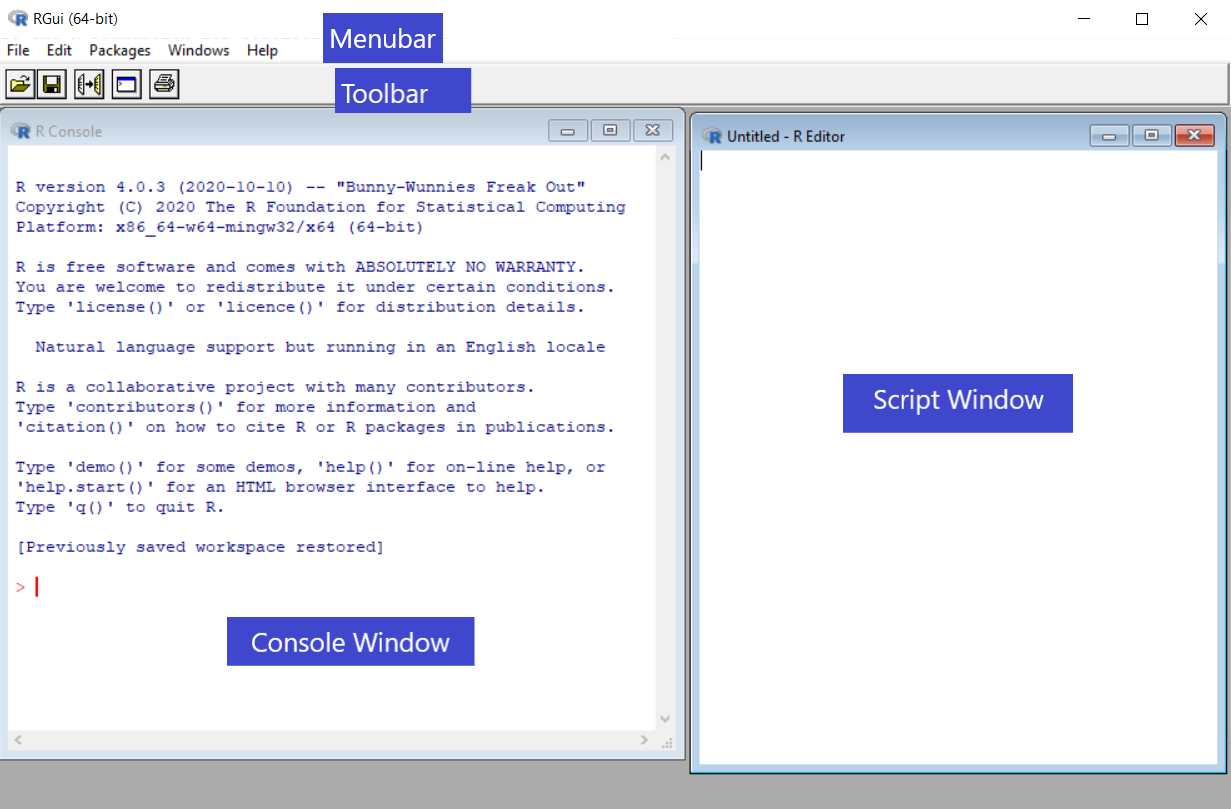
\includegraphics{fig_r0.png}

\hypertarget{instalasi-rstudio}{%
\section{\texorpdfstring{Instalasi
\emph{RStudio}}{Instalasi RStudio}}\label{instalasi-rstudio}}

Pada tahap awal, pemula memerlukan wahana \emph{platform} bantuan dalam
menjalankan bahasa \emph{R}. Salah satu pilihan \emph{platform} bantuan
adalah \emph{RStudio}. Dan, di bawah ini adalah langkah-langkah
sederhana untuk melakukan instalasi \emph{RStudi}.

\begin{itemize}
\tightlist
\item
  kunjungi situs: \url{https://www.rstudio.com}.
\item
  unduh \emph{RStudio IDE}\footnote{\emph{IDE (Integrated Development
    Environment)}: perangkat lunak atau program sebagai wadah/lingkungan
    yang mempermudah pelaksanaan pemrograman.}:
  \url{https://rstudio.com/products/rstudio/download/}.

  \begin{itemize}
  \tightlist
  \item
    versi pada 26/12/2020: \emph{RStudio Desktop 1.3.1093},
  \item
    versi ini mensyaratkan perlunya \emph{R} versi \emph{R3.0.1+} atau
    lebih.
  \end{itemize}
\end{itemize}

\emph{RStudio} telah terpasang dalam perangkat/mesin, serta siap
membantu dan mempermudah penggunaan bahasa \emph{R}.

\begin{quote}
Apakah \emph{RStudio} wajib dipasang? TIDAK, namun sebagaimana fungsinya
(sebagai \emph{IDE}), maka \emph{RStudio} dapat mempermudah telaah data
dan/atau proses pemrograman dengan \emph{R}. Tetapi, \emph{R} wajib
terpasang dalam perangkat, agar dapat menjalankan \emph{RStudio}.
\end{quote}

Berikut tampilan antarmuka \emph{RStudio}.

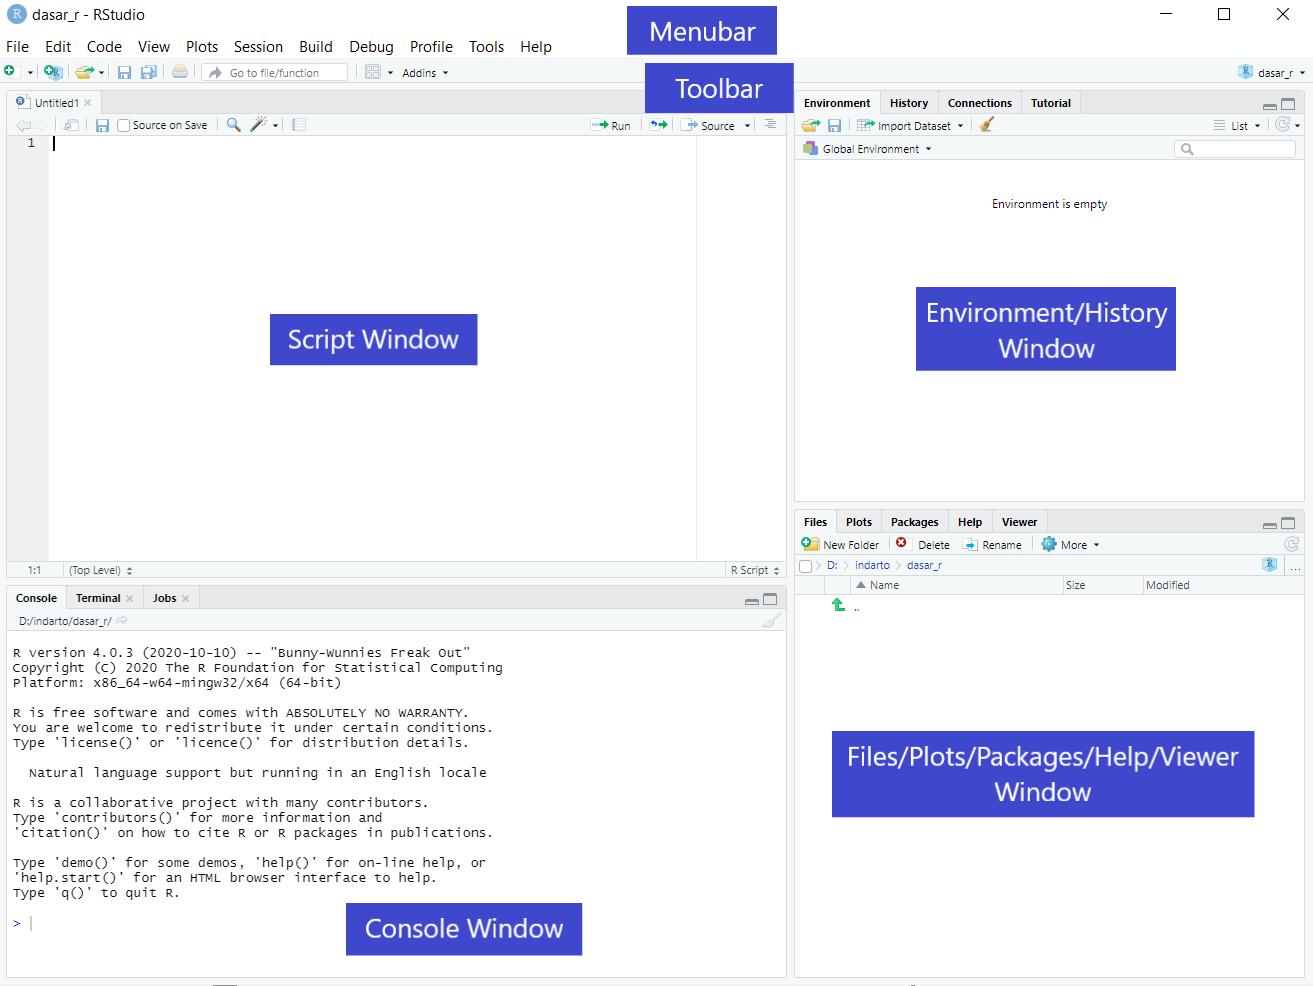
\includegraphics{fig_rstudio.png}

~

Bahasa \emph{R} telah dapat dijalankan, baik langsung melalui aplikasi
\emph{R} maupun dengan bantuan \emph{RStudio}.

\hypertarget{jalankanr}{%
\section{\texorpdfstring{Menjalankan \emph{R} dan/atau
\emph{RStudio}}{Menjalankan R dan/atau RStudio}}\label{jalankanr}}

Setelah proses instalasi berhasil, saatnya membuka dan menjalankan
aplikasi, baik melalui \emph{R} langsung maupun melalui bantuan
\emph{Rstudio}.

Mari memulai perkenalan dan percakapan dengan bahasa \emph{R}, melalui
beberapa contoh sintaks sederhana di bawah ini.

\begin{itemize}
\tightlist
\item
  membuat (\emph{assignment}) peubah atau \emph{variable}.

  \begin{itemize}
  \tightlist
  \item
    \emph{assignment} umumnya menggunakan tanda \texttt{"\textless{}-"}
    atau \texttt{"="}.
  \item
    sintaks dasar membuat peubah.
  \end{itemize}
\end{itemize}

\begin{Shaded}
\begin{Highlighting}[]
\NormalTok{nama_peubah <-}\StringTok{ }\NormalTok{nilai_peubah}
\end{Highlighting}
\end{Shaded}

\begin{itemize}
\tightlist
\item
  beberapa contoh pembuatan peubah.

  \begin{itemize}
  \tightlist
  \item
    membuat peubah bernama \texttt{"salam"}, yang berisi kata
    \texttt{"Assalaamuálaikum"}.
  \end{itemize}
\end{itemize}

\begin{Shaded}
\begin{Highlighting}[]
\NormalTok{salam <-}\StringTok{ "Assalaamuálaikum"}

\KeywordTok{print}\NormalTok{(salam)  }\CommentTok{# sintaks 'print()' untuk mencetak}
\end{Highlighting}
\end{Shaded}

\begin{verbatim}
## [1] "Assalaamuálaikum"
\end{verbatim}

\begin{itemize}
\tightlist
\item
  contoh lain.
\end{itemize}

\begin{Shaded}
\begin{Highlighting}[]
\NormalTok{nama <-}\StringTok{ "Fulan"}
\NormalTok{usia <-}\StringTok{ }\DecValTok{25}
\KeywordTok{print}\NormalTok{(}\KeywordTok{c}\NormalTok{(nama, }\StringTok{"berumur"}\NormalTok{, usia, }\StringTok{"tahun."}\NormalTok{))}
\end{Highlighting}
\end{Shaded}

\begin{verbatim}
## [1] "Fulan"   "berumur" "25"      "tahun."
\end{verbatim}

\begin{Shaded}
\begin{Highlighting}[]
\KeywordTok{cat}\NormalTok{(nama, }\StringTok{"berumur"}\NormalTok{, usia, }\StringTok{"tahun."}\NormalTok{)  }\CommentTok{# cat: concatenate}
\end{Highlighting}
\end{Shaded}

\begin{verbatim}
## Fulan berumur 25 tahun.
\end{verbatim}

Kita telah mulai berkenalan dengan bahasa \emph{R}. Juga, kita telah
memastikan bahwa perangkat/mesin telah dapat menjalankan bahasa \emph{R}
dengan baik.

\hypertarget{pilihan-lain}{%
\section{Pilihan Lain}\label{pilihan-lain}}

Selain langsung melalui aplikasi \emph{R} maupun bantuan \emph{RStudio},
bahasa \emph{R} juga dapat dijalankan melalui beberapa \emph{notebook
platform/environment}, tanpa melakukan proses instalasi dalam
perangkat/mesin. Di bawah ini disajikan beberapa
\emph{notebook}\footnote{\emph{Notebook} atau \emph{notebook document}
  merupakan \emph{platform} yang mampu memadukan antara pengkodean
  (penulisan kode, menjalankan kode, dan hasil pengkodean, termasuk
  visualisasi data), dengan narasi teks, penulisan karakter matematika,
  dan media lain dalam satu dokumen.}, yang dapat dimanfaatkan untuk
menjalankan bahasa \emph{R}, baik yang berdiri-sendiri maupun yang
berbasis \emph{web/cloud}.

\textbf{\emph{a. Jupyter Notebook}}

\begin{itemize}
\tightlist
\item
  \emph{Jupyter notebook} dapat dipasang dan dijalankan tersendiri,
  dengan langkah-langkah yang tersedia di tautan berikut:
  \url{https://jupyter.org/install}.
\item
  atau sebagai bagian dari \emph{Anaconda toolkit}, yang dapat diunduh
  di sini: \url{https://www.anaconda.com/products/individual}.
\item
  dapat dijalankan di luar jaringan (luring) untuk menjalankan
  \emph{Jupyter}.
\end{itemize}

\begin{quote}
Dinamakan \emph{Jupyter}, karena pada awalnya dikembangkan untuk
mendukung penggunaan bahasa program \textbf{\emph{Ju}}lia -
\textbf{\emph{Pyt}}hon - \textbf{\emph{R}}.
\end{quote}

\newpage

\textbf{\emph{b. Google Colaboratory Notebook (Google Colab)}}

\begin{itemize}
\tightlist
\item
  merupakan \emph{platform} gratis berbasis \emph{Jupyter notebook} yang
  dijalankan sepenuh melalui \emph{cloud}.
\item
  \emph{Google Colab} sebenarnya dirancang untuk menjalankan bahasa
  \emph{Python}.
\item
  namun demikian, \emph{Google Colab} dapat menjalankan bahasa \emph{R},
  dengan mengakses melalui tautan berikut:

  \begin{itemize}
  \tightlist
  \item
    \url{https://colab.research.google.com/\#create=true\&language=r},
    atau
  \item
    \url{https://colab.to/r}.
  \end{itemize}
\item
  perlu masuk dalam jaringan (daring) untuk menjalankan \emph{Google
  Colab}.
\end{itemize}

\textbf{\emph{c.~Kaggle Notebook}}

\begin{itemize}
\tightlist
\item
  \emph{Kaggle} menyediakan fasilitas pengkodean \emph{R} ini, dengan
  mengakses melaui tautan ini: \url{https://www.kaggle.com/notebooks}.
\item
  perlu masuk dalam jaringan (daring) untuk menjalankan \emph{Kaggle
  Notebook}.
\end{itemize}

\textbf{\emph{d.~Azure Notebooks}}\footnote{Dalam situs resminya, yang
  kami akses pada 30-Desember-2020, diberikan pengumuman sebagai
  berikut: ``\emph{The Azure Notebooks preview will be retired on
  January 15th, 2021, and all user data will be destroyed. Please
  download your user data before then. To execute notebooks or create
  new notebook content, learn about our other notebooks experiences at
  Microsoft}''. Saat ini, \emph{Microsoft} mengembangkan beberapa
  \emph{platform} layanan, antara lain: \emph{Visual Code}, \emph{Github
  Codespace}, \emph{Azure Machine Learning}, maupun \emph{Azure Lab}.
  Pilihan layanan tersebut dapat diakses di sini:
  \url{https://notebooks.azure.com/Content/alternatives.html}.}

\begin{itemize}
\tightlist
\item
  \emph{Microsoft} mengembangkan \emph{Azure Notebooks} sebagai
  \emph{platform} bahasa program berbasis \emph{Jupyter Notebook}, yang
  dapat digunakan untuk menjalankan bahasa R.
\item
  \emph{Azure Notebooks} dapat diakses di sini:
  \url{https://notebooks.azure.com/}.
\item
  perlu masuk dalam jaringan (daring) untuk menjalankan \emph{Azure
  Notebook}.
\end{itemize}

\textbf{\emph{e. Amazon SageMaker}}

\begin{itemize}
\tightlist
\item
  \emph{Amazon} juga mengembangkan \emph{cloud platform} sebagai
  \emph{Amazon Web Services (AWS)}.
\item
  salah satu fasilitas \emph{AWS} adalah \emph{Amazon SageMaker}, yang
  berbasis \emph{Jupyter Notebook} dan dapat digunakan untuk menjalankan
  bahasa \emph{R} melalui tautan:
  \url{https://aws.amazon.com/sagemaker/}.
\item
  perlu masuk dalam jaringan (daring) untuk menjalankan \emph{Amazon
  SageMaker}.
\end{itemize}

\textbf{\emph{f.~IBM DataPlatform Notebooks}}

\begin{itemize}
\tightlist
\item
  Pilihan lain untuk menjalankan \emph{R} adalah \emph{IBM DataPlatfrom
  Notebook} yang dikembangkan oleh \emph{IBM Watson Data Platform and
  Data Science Experince (DSX)}.
\item
  fasilitas ini dapat dinikmati melalui tautan berikut:
  \url{https://dataplatform.cloud.ibm.com/}.
\item
  perlu masuk dalam jaringan (daring) untuk menjalankan \emph{IBM
  Notebook}.
\end{itemize}

~

Dengan telah terpasangnya \emph{R}, maka telaah data dan/atau
pemrograman sudah dapat dilakukan dengan bahasa \emph{R} dalam
perangkat. \emph{RStudio} juga dapat dijalankan untuk mempermudah proses
tersebut. Selain itu, beberapa pilihan \emph{notebooks platform}, baik
yang berdiri-sendiri maupun \emph{web-based/cloud}, terbuka luas untuk
menjembatani kita dalam menjalankan bahasa \emph{R}.

Selain itu, kita telah berkenalan dengan beberapa sintaks
(\emph{script}) dalam bahasa \emph{R}. Bab-bab selanjutnya membahas
telaah data dan \emph{dataset} dengan bahasa \emph{R}.

\newpage

\hypertarget{dasar-penyiapan-direktori-kerja-dan-dataset}{%
\chapter{\texorpdfstring{Dasar Penyiapan Direktori Kerja dan
\emph{Dataset}}{Dasar Penyiapan Direktori Kerja dan Dataset}}\label{dasar-penyiapan-direktori-kerja-dan-dataset}}

Bab ini menyajikan beberapa persiapan awal sebelum melakukan telaah
data. Persiapan ini ditujukan untuk mempermudah langkah-langkah
selanjutnya. Bahasan meliputi penyiapan direktori kerja (\emph{working
directory - wd}), penyiapan \emph{file} data yang akan ditelaah,
penyiapan \emph{dataset} agar dapat dibaca oleh bahasa \emph{R}, serta
pengenalan beberapa tipe data atomik bahasa \emph{R}.

\hypertarget{penyiapan-working-directory-wd}{%
\section{\texorpdfstring{Penyiapan \emph{Working Directory
(wd)}}{Penyiapan Working Directory (wd)}}\label{penyiapan-working-directory-wd}}

Sebelum menelaah data lebih lanjut, kita menyiapkan \emph{folder}
direktori kerja (\emph{wd}) terlebih dahulu. \emph{Folder} ini merupakan
\emph{working directory} yang dipergunakan untuk menyimpan seluruh file
yang diperlukan dan akan dihasilkan dalam dalam proyek (\emph{project})
kita.

\begin{itemize}
\tightlist
\item
  melihat posisi/jalur (\emph{path}) \emph{folder} saat ini.
\end{itemize}

\begin{Shaded}
\begin{Highlighting}[]
\KeywordTok{getwd}\NormalTok{()  }\CommentTok{# membaca posisi folder dimana mesin bekerja saat ini}
\end{Highlighting}
\end{Shaded}

\begin{itemize}
\tightlist
\item
  mengatur \emph{path} pada \emph{folder} \emph{wd} yang kita ingingkan.
\end{itemize}

\begin{Shaded}
\begin{Highlighting}[]
\KeywordTok{setwd}\NormalTok{(}\StringTok{"D:/indarto/r_boekoe"}\NormalTok{)  }\CommentTok{# contoh folder yang disiapkan}
\end{Highlighting}
\end{Shaded}

\begin{itemize}
\tightlist
\item
  membaca data apa saja yang berada pada \emph{folder wd}.
\end{itemize}

\begin{Shaded}
\begin{Highlighting}[]
\KeywordTok{dir}\NormalTok{()}
\end{Highlighting}
\end{Shaded}

\hypertarget{penyiapan-file-data}{%
\section{\texorpdfstring{Penyiapan \emph{File}
Data}{Penyiapan File Data}}\label{penyiapan-file-data}}

Untuk mempermudah dan menyederhanakan pemahaman, buku/modul ini telah
menyiapkan data jadi\footnote{Topik tentang pembuatan data, konversi
  tipe dan format data, penggalian data (\emph{data mining}), dan
  lain-lain, belum dibahas dalam buku/modul ini; namun, sangat
  disarankan untuk dipelajari lebih lanjut.}, untuk dipergunakan pada
latihan-latihan pada Bab-bab selanjutnya. Data latihan ini adalah
\textbf{\emph{``tree.csv''}} dan berbentuk format
\textbf{\emph{.csv}}\footnote{\emph{Comma Separated Values}, kadang
  disebut \emph{Character Separated Values} atau \emph{Comma Delimited
  File}, merupakan format \emph{file} dalam bentuk teks dimana data
  disimpan dan dipisahkan dengan tanda tertentu (koma, titik koma,
  \emph{tab}, dan lain-lain)}, dengan tanda koma (,) sebagai
\emph{delimiter}. Data latihan ini dapat diunduh melalui tautan berikut:
\url{https://indarto.weebly.com/uploads/7/9/1/0/7910347/tree.csv}.

\begin{itemize}
\tightlist
\item
  sekilas tentang isi data \textbf{``tree.csv''}.

  \begin{itemize}
  \tightlist
  \item
    data merupakan pengamatan dari 95 pohon.

    \begin{itemize}
    \tightlist
    \item
      terdiri dari 5 kelompok, yaitu kelompok 7, kelompok 12, kelompok
      15, kelompok 31, dan kelompok 37.
    \item
      kelompok ini berada pada kolom pertama ``treeID''.
    \end{itemize}
  \item
    \emph{variable} yang diamati meliputi:

    \begin{itemize}
    \tightlist
    \item
      ``Age'': umur pohon.
    \item
      ``DBH'': \emph{diameter at breast height} (diameter pada
      ketinggian 4.5 kaki dari permukaan tanah).
    \item
      ``Height'': tinggi pohon.
    \item
      ``Volume'': volume kayu.
    \end{itemize}
  \end{itemize}
\item
  silahkan mengunduh \emph{file} data latihan tersebut
  \href{https://indarto.weebly.com/uploads/7/9/1/0/7910347/tree.csv}{di
  sini}.
\item
  simpan dalam \emph{folder wd} yang telah kita siapkan di atas.
\item
  periksa dan pastikan kembali bahwa \emph{file} latihan tersebut telah
  siap di \emph{folder wd}.
\end{itemize}

\begin{Shaded}
\begin{Highlighting}[]
\KeywordTok{dir}\NormalTok{()}
\end{Highlighting}
\end{Shaded}

Kita telah menyiapkan \emph{folder wd} dan memastikan bahwa data telah
berada pada \emph{folder wd} tersebut.

\hypertarget{penyiapan-dataset-bagi-r}{%
\section{\texorpdfstring{Penyiapan \emph{Dataset} bagi
\emph{R}}{Penyiapan Dataset bagi R}}\label{penyiapan-dataset-bagi-r}}

Data latihan \emph{``tree.csv''} telah siap dan berada pada \emph{folder
wd} yang diinginkan. Namun, data tersebut masih berada dalam format
ekstensi \emph{``.csv''}, sehingga perlu di-\emph{import} menjadi
\emph{dataframe} untuk bisa dibaca oleh bahasa \emph{R}\footnote{Sebagai
  bahasa program, \emph{R environment} mampu membaca, menuliskan,
  meng-\emph{import}, atau meng-\emph{export} data dari/ke berbagai tipe
  format \emph{file} (antara lain: \emph{.csv}, \emph{.xlsx},
  \emph{.txt}, \emph{.rds}, \emph{.xml}, \emph{.json}, maupun dari
  situs, dan lain-lain). Buku/modul ini tidak memberikan pembahasan
  khusus tentang ini, namun sangat disarankan untuk dapat dipelajari
  lebih lanjut.}. Dari sesi di atas, \emph{file}
\textbf{\emph{tree.csv}} telah disimpan dalam \emph{wd}.

\begin{itemize}
\tightlist
\item
  membuat (\emph{assignment}) \emph{dataset}, sintaks:
  \texttt{nama\_dataset\ \textless{}-\ isi\_dataset}.

  \begin{itemize}
  \tightlist
  \item
    membuat \emph{dataset} bernama \textbf{``pohon''} yang berisi data
    dari \emph{file} \textbf{``tree.csv''}.
  \end{itemize}
\end{itemize}

\begin{Shaded}
\begin{Highlighting}[]
\NormalTok{pohon <-}\StringTok{ }\KeywordTok{read.csv}\NormalTok{(}\StringTok{"tree.csv"}\NormalTok{)}
\end{Highlighting}
\end{Shaded}

\begin{itemize}
\tightlist
\item
  R juga bisa langsung mengakses data langsung dari sumber situsnya
  (perlu terhubung ke internet).
\end{itemize}

\begin{Shaded}
\begin{Highlighting}[]
\NormalTok{pohon <-}\StringTok{ }\KeywordTok{read.csv}\NormalTok{(}\StringTok{"https://indarto.weebly.com/uploads/7/9/1/0/7910347/tree.csv"}\NormalTok{)}
\end{Highlighting}
\end{Shaded}

\begin{itemize}
\tightlist
\item
  bisa menambahkan \emph{parameter} ``header=T'' karena baris pertama
  pada data \textbf{``tree.csv''} adalah \emph{header} (nama kolom).
\end{itemize}

\begin{Shaded}
\begin{Highlighting}[]
\NormalTok{pohon <-}\StringTok{ }\KeywordTok{read.csv}\NormalTok{(}\StringTok{"tree.csv"}\NormalTok{, }\DataTypeTok{header =}\NormalTok{ T)}
\end{Highlighting}
\end{Shaded}

\begin{itemize}
\tightlist
\item
  memeriksa dan memastikan bahwa \emph{dataset} \textbf{``pohon''} telah
  ada pada \emph{folder wd}.
\end{itemize}

\begin{Shaded}
\begin{Highlighting}[]
\KeywordTok{ls}\NormalTok{()}
\end{Highlighting}
\end{Shaded}

\begin{itemize}
\tightlist
\item
  memeriksa \emph{class} dari data \emph{pohon}.

  \begin{itemize}
  \tightlist
  \item
    sintaks: \texttt{class()}.
  \end{itemize}
\end{itemize}

\begin{Shaded}
\begin{Highlighting}[]
\KeywordTok{class}\NormalTok{(pohon)}
\end{Highlighting}
\end{Shaded}

\begin{verbatim}
## [1] "data.frame"
\end{verbatim}

\emph{File} data \emph{tree.csv} yang awalnya berbentuk \emph{csv},
sekarang berbentuk kelas \emph{dataframe}\footnote{\emph{Dataframe}
  merupakan salah satu bentuk \emph{R-objects}. Beberapa jenis
  \emph{R-objects}, antara lain: \emph{vectors}, \emph{lists},
  \emph{matrices}, \emph{arrays}, \emph{factors}, dan \emph{dataframe}.
  Pilihan \emph{R-objects} tersebut, memungkinkan pengguna dalam memilih
  kelas \emph{dataset} yang sesuai untuk menyimpan datanya. Buku/modul
  ini tidak membahas jenis \emph{R-objects} tersebut; namun, sangat
  disarankan untuk dipelajari lebih lanjut.} dan siap dijalankan oleh
bahasa \emph{R}.

\hypertarget{tipedata}{%
\section{Pengenalan Tipe Data}\label{tipedata}}

Dari peubah-peubah yang dibuat pada Bab sebelumnya, sesi
\protect\hyperlink{jalankanr}{Menjalankan \emph{R} dan/atau
\emph{RStudio}} , kita mengenal beberapa tipe data. Bahasa R mengenal
tipe-tipe data, disebut sebagai \textbf{\emph{atomic data types}},
antara lain: \textbf{\emph{character}}, \textbf{\emph{numeric}},
\textbf{\emph{logical}}, \emph{complex} dan \emph{raw}. Tiga
\emph{atomic data types} diperkenalkan di bawah ini. Sintaks:
\texttt{class()} atau \texttt{typeof()}.

\textbf{a. Data Karakter (\emph{character} atau \emph{string})}

\begin{itemize}
\tightlist
\item
  peubah bukan angka.
\item
  data karakter dituliskan di dalam tanda petik (``data\_karakter'').

  \begin{itemize}
  \tightlist
  \item
    contoh, peubah ``salam'' dan ``nama'' di atas merupakan data
    karakter.
  \end{itemize}
\end{itemize}

\begin{Shaded}
\begin{Highlighting}[]
\KeywordTok{class}\NormalTok{(salam)}
\end{Highlighting}
\end{Shaded}

\begin{verbatim}
## [1] "character"
\end{verbatim}

\begin{Shaded}
\begin{Highlighting}[]
\KeywordTok{class}\NormalTok{(nama)}
\end{Highlighting}
\end{Shaded}

\begin{verbatim}
## [1] "character"
\end{verbatim}

\begin{itemize}
\tightlist
\item
  angka jika ditulis dalam tanda petik, maka merupakan data karakter.
\end{itemize}

\begin{Shaded}
\begin{Highlighting}[]
\KeywordTok{class}\NormalTok{(usia)}
\end{Highlighting}
\end{Shaded}

\begin{verbatim}
## [1] "numeric"
\end{verbatim}

\begin{Shaded}
\begin{Highlighting}[]
\KeywordTok{class}\NormalTok{(}\StringTok{"25"}\NormalTok{)}
\end{Highlighting}
\end{Shaded}

\begin{verbatim}
## [1] "character"
\end{verbatim}

\textbf{b. Data Numerik (\emph{numeric})}

\begin{itemize}
\tightlist
\item
  peubah angka.
\item
  dapat berupa angka bulat (tanpa desimal).
\end{itemize}

\begin{Shaded}
\begin{Highlighting}[]
\KeywordTok{class}\NormalTok{(usia)}
\end{Highlighting}
\end{Shaded}

\begin{verbatim}
## [1] "numeric"
\end{verbatim}

\begin{itemize}
\tightlist
\item
  dapat berupa angka desimal.
\end{itemize}

\begin{Shaded}
\begin{Highlighting}[]
\NormalTok{ipk <-}\StringTok{ }\FloatTok{3.45}
\KeywordTok{class}\NormalTok{(ipk)}
\end{Highlighting}
\end{Shaded}

\begin{verbatim}
## [1] "numeric"
\end{verbatim}

\begin{itemize}
\tightlist
\item
  data numerik memungkinkan untuk diolah dengan operasi aritmatika
  (penambahan, pengurangan, perkalian, pembagian, pangkat, dan
  lain-lain).
\end{itemize}

\begin{Shaded}
\begin{Highlighting}[]
\NormalTok{next5years <-}\StringTok{ }\NormalTok{usia }\OperatorTok{+}\StringTok{ }\DecValTok{5}  \CommentTok{# usia lima tahun ke depan}
\KeywordTok{print}\NormalTok{(next5years)}
\end{Highlighting}
\end{Shaded}

\begin{verbatim}
## [1] 30
\end{verbatim}

\begin{Shaded}
\begin{Highlighting}[]
\KeywordTok{class}\NormalTok{(next5years)}
\end{Highlighting}
\end{Shaded}

\begin{verbatim}
## [1] "numeric"
\end{verbatim}

\textbf{c.~Data Logika (\emph{logical} atau \emph{boolean})}

\begin{itemize}
\tightlist
\item
  bernilai \emph{TRUE} (\emph{T}) atau \emph{FALSE} (\emph{F}).
\end{itemize}

\begin{Shaded}
\begin{Highlighting}[]
\NormalTok{lulus <-}\StringTok{ }\NormalTok{ipk }\OperatorTok{>=}\StringTok{ }\FloatTok{2.75}
\KeywordTok{print}\NormalTok{(lulus)}
\end{Highlighting}
\end{Shaded}

\begin{verbatim}
## [1] TRUE
\end{verbatim}

\begin{Shaded}
\begin{Highlighting}[]
\KeywordTok{class}\NormalTok{(lulus)}
\end{Highlighting}
\end{Shaded}

\begin{verbatim}
## [1] "logical"
\end{verbatim}

Data kategori (\emph{categorical}) akan disajikan contohnya pada akhir
sesi \protect\hyperlink{tinjauan-dataset}{Tinjauan \emph{Dataset}}.
Sedangkan, tipe data atomik lain (misalkan: \emph{complex},
\emph{integer}, \emph{real}, atau \emph{raw}) tidak dibahas dalam
buku/modul ini; namun, disarankan untuk dapat dipelajari lebih lanjut.

\newpage

\hypertarget{dasar-tinjauan-data}{%
\chapter{Dasar Tinjauan Data}\label{dasar-tinjauan-data}}

Kita telah menyiapkan direktori kerja dan \emph{dataset} yang sudah
dapat dibaca oleh bahasa \emph{R}. Selanjutnya, Bab ini mengenalkan
dasar-dasar untuk meninjau isi dari \emph{dataset} kita. Bahasan
meliputi tinjauan umum \emph{dataset}, tinjauan baris dan kolom (atau
dikenal sebagai proses \emph{subsetting}, \emph{slicing} atau
\emph{extracting}), serta modifikasi sederhana terhadap data (penambahan
dan penghapusan dan kolom).

\hypertarget{tinjauan-dataset}{%
\section{\texorpdfstring{Tinjauan
\emph{Dataset}}{Tinjauan Dataset}}\label{tinjauan-dataset}}

\emph{Dataset} berisi sekumpulan data, dalam bentuk baris dan kolom.
\emph{Dataset} dapat terdiri dari satu atau lebih baris dan satu atau
lebih kolom. Dengan demikian, \emph{dataset} paling tidak mempunyai satu
baris dan satu kolom.

Dalam \emph{dataset} ``pohon'' yang digunakan dalam latihan buku/modul
ini, satu kolom mewakili satu \emph{variable}, sehingga pada kolom yang
sama bertipe data yang sama.

Selanjutnya, kita melakukan tinjauan singkat terhadap \emph{dataset}
kita.

\begin{itemize}
\tightlist
\item
  dimensi \emph{dataset}, sintaks: \texttt{dim()}.
\end{itemize}

\begin{Shaded}
\begin{Highlighting}[]
\KeywordTok{dim}\NormalTok{(pohon)  }\CommentTok{# dataset 'pohon' terdiri dari 95 baris dan 5 kolom}
\end{Highlighting}
\end{Shaded}

\begin{verbatim}
## [1] 95  5
\end{verbatim}

\begin{itemize}
\tightlist
\item
  nama kolom \emph{header} pada \emph{dataset}, sintaks:
  \texttt{names()} atau \texttt{colnames()}.
\end{itemize}

\begin{Shaded}
\begin{Highlighting}[]
\KeywordTok{names}\NormalTok{(pohon)  }\CommentTok{# memberikan hasil yang sama}
\end{Highlighting}
\end{Shaded}

\begin{verbatim}
## [1] "treeID" "Age"    "DBH"    "Height" "Volume"
\end{verbatim}

\begin{Shaded}
\begin{Highlighting}[]
\KeywordTok{colnames}\NormalTok{(pohon)}
\end{Highlighting}
\end{Shaded}

\begin{verbatim}
## [1] "treeID" "Age"    "DBH"    "Height" "Volume"
\end{verbatim}

Terlihat bahwa \emph{dataset} ``pohon'' mempunyai 5 kolom atau
\emph{header} atau \emph{variable}, yaitu: ``treeID'': kolom 1, ``Age'':
kolom 2, ``DBH'': kolom 3, ``Height'': kolom 4 dan ``Volume'': kolom 5.

\newpage

\begin{itemize}
\tightlist
\item
  struktur \emph{dataset}, sintaks: \texttt{str()}.
\end{itemize}

\begin{Shaded}
\begin{Highlighting}[]
\KeywordTok{str}\NormalTok{(pohon)}
\end{Highlighting}
\end{Shaded}

\begin{verbatim}
## 'data.frame':    95 obs. of  5 variables:
##  $ treeID: int  7 7 7 7 7 7 7 7 7 7 ...
##  $ Age   : int  2 3 4 5 6 7 8 9 10 11 ...
##  $ DBH   : num  0 0.35 1.73 4.29 6.59 ...
##  $ Height: num  0.7 1.6 2.6 3.6 4.6 5.5 6.6 7.6 8.4 8.9 ...
##  $ Volume: num  0 0 0.001 0.004 0.01 0.018 0.027 0.035 0.045 0.051 ...
\end{verbatim}

Sintaks \texttt{str()} menampilkan ringkasan struktur data, antara lain:
nama kolom/\emph{variable}, jumlah observasi, jumlah \emph{variables}
atau kolom, tipe data (\emph{integer}, \emph{numeric}, dll.) dan
ringkasan nilai dari setiap \emph{variable} atau kolom.

\begin{itemize}
\tightlist
\item
  ringkasan statistik \emph{dataset}, sintaks: \texttt{summary()}.
\end{itemize}

\begin{Shaded}
\begin{Highlighting}[]
\KeywordTok{summary}\NormalTok{(pohon)}
\end{Highlighting}
\end{Shaded}

\begin{verbatim}
##      treeID          Age          DBH             Height      
##  Min.   : 7.0   Min.   : 2   Min.   : 0.000   Min.   : 0.500  
##  1st Qu.:12.0   1st Qu.: 6   1st Qu.: 6.245   1st Qu.: 4.300  
##  Median :15.0   Median :11   Median :11.240   Median : 8.600  
##  Mean   :20.4   Mean   :11   Mean   : 9.656   Mean   : 8.058  
##  3rd Qu.:31.0   3rd Qu.:16   3rd Qu.:13.715   3rd Qu.:11.550  
##  Max.   :37.0   Max.   :20   Max.   :15.790   Max.   :15.400  
##      Volume       
##  Min.   :0.00000  
##  1st Qu.:0.00900  
##  Median :0.04500  
##  Mean   :0.05101  
##  3rd Qu.:0.08600  
##  Max.   :0.14800
\end{verbatim}

Sintaks \texttt{summary()} menampilkan ringkasan statistik dari setiap
\emph{variable} yang mengandung tipe data \emph{numeric} atau
\emph{non-character}. Ringkasan meliputi: nama kolom/\emph{variable},
\emph{minimum}, \emph{maximum}, \emph{median}, \emph{mean}, \emph{1st
quantile}, dan \emph{3rd quantile}.

\newpage

\begin{itemize}
\tightlist
\item
  melihat isi atau nilai data, sintaks: \texttt{head()} atau
  \texttt{tail()}.
\end{itemize}

\begin{Shaded}
\begin{Highlighting}[]
\KeywordTok{head}\NormalTok{(pohon)  }\CommentTok{# menampilkan isi 5 baris pertama}
\end{Highlighting}
\end{Shaded}

\begin{verbatim}
##   treeID Age  DBH Height Volume
## 1      7   2 0.00    0.7  0.000
## 2      7   3 0.35    1.6  0.000
## 3      7   4 1.73    2.6  0.001
## 4      7   5 4.29    3.6  0.004
## 5      7   6 6.59    4.6  0.010
## 6      7   7 8.38    5.5  0.018
\end{verbatim}

\begin{Shaded}
\begin{Highlighting}[]
\KeywordTok{tail}\NormalTok{(pohon)  }\CommentTok{# menampilkan 5 baris terakhir}
\end{Highlighting}
\end{Shaded}

\begin{verbatim}
##    treeID Age   DBH Height Volume
## 90     37  15 14.16   10.9  0.075
## 91     37  16 14.53   11.6  0.083
## 92     37  17 14.86   12.3  0.090
## 93     37  18 15.13   12.9  0.097
## 94     37  19 15.36   13.7  0.104
## 95     37  20 15.55   14.4  0.111
\end{verbatim}

Kita juga dapat mengatur jumlah baris yang akan ditampilkan, dengan
menambahkan angka sebagai \emph{parameter} pada sintaks \texttt{head()}
atau \texttt{tail()} di atas.

\begin{Shaded}
\begin{Highlighting}[]
\KeywordTok{head}\NormalTok{(pohon, }\DecValTok{7}\NormalTok{)  }\CommentTok{# menampilkan 7 baris pertama}
\end{Highlighting}
\end{Shaded}

\begin{verbatim}
##   treeID Age  DBH Height Volume
## 1      7   2 0.00    0.7  0.000
## 2      7   3 0.35    1.6  0.000
## 3      7   4 1.73    2.6  0.001
## 4      7   5 4.29    3.6  0.004
## 5      7   6 6.59    4.6  0.010
## 6      7   7 8.38    5.5  0.018
## 7      7   8 9.92    6.6  0.027
\end{verbatim}

\begin{Shaded}
\begin{Highlighting}[]
\KeywordTok{tail}\NormalTok{(pohon, }\DecValTok{3}\NormalTok{)  }\CommentTok{# menampilkan 3 baris terakhir}
\end{Highlighting}
\end{Shaded}

\begin{verbatim}
##    treeID Age   DBH Height Volume
## 93     37  18 15.13   12.9  0.097
## 94     37  19 15.36   13.7  0.104
## 95     37  20 15.55   14.4  0.111
\end{verbatim}

\newpage

\textbf{Data Kategori (\emph{categorical variable})}

Pada sesi \protect\hyperlink{tipedata}{Mengenal Tipe Data}, kita telah
mengenal tiga tipe data atomik, yaitu \emph{character}, \emph{numeric},
dan \emph{logical}. Dari \emph{dataset} ``pohon'' di atas, kita menambah
pengenalan tentang tipe data kategori. Dengan mencermati hasil sintaks
\texttt{head(pohon)} dan \texttt{tail(pohon)} di atas, terlihat bahwa
\emph{variable} ``treeID'' terkategorikan dalam beberapa kelompok.

\begin{itemize}
\tightlist
\item
  sintaks untuk memerika nilai unik dari variable tertentu:
  \texttt{unique()}.
\item
  memeriksa struktur \emph{variable} ``treeID''.
\end{itemize}

\begin{Shaded}
\begin{Highlighting}[]
\KeywordTok{str}\NormalTok{(pohon}\OperatorTok{$}\NormalTok{treeID)  }\CommentTok{# 'treeID' berjumlah 95 observasi.}
\end{Highlighting}
\end{Shaded}

\begin{verbatim}
##  int [1:95] 7 7 7 7 7 7 7 7 7 7 ...
\end{verbatim}

\begin{itemize}
\tightlist
\item
  memeriksa nilai unik atau kelompok kategori ``treeID''.
\end{itemize}

\begin{Shaded}
\begin{Highlighting}[]
\KeywordTok{unique}\NormalTok{(pohon}\OperatorTok{$}\NormalTok{treeID)}
\end{Highlighting}
\end{Shaded}

\begin{verbatim}
## [1]  7 12 15 31 37
\end{verbatim}

Walaupun ``treeID'' mempunyai 95 obervasi, \emph{variable} ini mempunyai
5 kategori/kelompok, yaitu: 7, 12, 15, 31, 37.

\hypertarget{tinjauan-baris-dan-kolom}{%
\section{Tinjauan Baris dan Kolom}\label{tinjauan-baris-dan-kolom}}

Kita telah melakukan tinjauan singkat terhadap \emph{dataset} ``pohon''
(struktur, ringkasan statistik, dan isi). Kita akan melakukan tinjauan
lebih lanjut terhadap baris atau kolom tertentu, termasuk ekstraksi
(\emph{extracting/slicing}) terhadap \emph{dataset} kita.

\begin{itemize}
\tightlist
\item
  sintaks dasar untuk melakukan \emph{slicing} baris/kolom tertentu dari
  \emph{dataset}: \texttt{nama\_*dataset*{[}baris\ ke-,\ kolom\ ke-{]}}.
\item
  ingat kembali bahwa \emph{dataset} ``pohon'' terdiri dari 95 baris dan
  5 kolom.
\end{itemize}

\begin{Shaded}
\begin{Highlighting}[]
\KeywordTok{dim}\NormalTok{(pohon)}
\end{Highlighting}
\end{Shaded}

\begin{verbatim}
## [1] 95  5
\end{verbatim}

\textbf{a. Ekstrak/iris baris}

\begin{itemize}
\tightlist
\item
  sintaks: \texttt{dataset{[}baris\ ke-,\ {]}}.
\item
  mengekstrak baris ke-3, untuk seluruh kolom.
\end{itemize}

\begin{Shaded}
\begin{Highlighting}[]
\NormalTok{pohon[}\DecValTok{3}\NormalTok{, ]}
\end{Highlighting}
\end{Shaded}

\begin{verbatim}
##   treeID Age  DBH Height Volume
## 3      7   4 1.73    2.6  0.001
\end{verbatim}

\begin{itemize}
\tightlist
\item
  mengesktrak baris ke 1-5 untuk seluruh kolom.
\end{itemize}

\begin{Shaded}
\begin{Highlighting}[]
\NormalTok{pohon[}\DecValTok{1}\OperatorTok{:}\DecValTok{5}\NormalTok{, ]  }\CommentTok{# hasilnya sama dengan sintaks 'head()'}
\end{Highlighting}
\end{Shaded}

\begin{verbatim}
##   treeID Age  DBH Height Volume
## 1      7   2 0.00    0.7  0.000
## 2      7   3 0.35    1.6  0.000
## 3      7   4 1.73    2.6  0.001
## 4      7   5 4.29    3.6  0.004
## 5      7   6 6.59    4.6  0.010
\end{verbatim}

\textbf{b. Ekstrak/iris kolom}

\begin{itemize}
\tightlist
\item
  sintaks: \texttt{dataset{[}\ ,\ kolom\ ke-{]}}.
\item
  ingat kembali bahwa \emph{dataset} ``pohon'' mempunyai 5 kolom atau
  \emph{variables}, yaitu: kolom ke-1 = ``treeID'', kolom ke-2 =
  ``Age'', kolom ke-3 = ``DBH'', kolom ke-4 = ``Height'', dan kolom ke-5
  = ``Volume''.
\end{itemize}

\begin{Shaded}
\begin{Highlighting}[]
\KeywordTok{colnames}\NormalTok{(pohon)}
\end{Highlighting}
\end{Shaded}

\begin{verbatim}
## [1] "treeID" "Age"    "DBH"    "Height" "Volume"
\end{verbatim}

\begin{itemize}
\tightlist
\item
  mengekstrak kolom ke-3, untuk seluruh baris.
\end{itemize}

\begin{Shaded}
\begin{Highlighting}[]
\KeywordTok{options}\NormalTok{(}\DataTypeTok{width =} \DecValTok{70}\NormalTok{)  }\CommentTok{# sintaks ini tidak harus ada}
\NormalTok{pohon[, }\DecValTok{3}\NormalTok{]}
\end{Highlighting}
\end{Shaded}

\begin{verbatim}
##  [1]  0.00  0.35  1.73  4.29  6.59  8.38  9.92 10.86 11.66 11.97 12.40
## [12] 12.97 13.57 13.88 14.12 14.57 14.94 15.41 15.79  0.00  0.00  1.36
## [23]  3.23  5.21  6.71  8.08  8.99  9.77 10.19 10.81 11.41 12.05 12.40
## [34] 12.74 13.06 13.38 13.69 13.94  0.00  0.05  1.60  3.51  5.90  7.61
## [45]  9.02  9.80 10.67 11.14 11.93 12.60 13.30 13.66 14.00 14.41 14.86
## [56] 15.22 15.57  0.00  0.51  1.25  3.16  5.60  7.41  8.82  9.82 10.82
## [67] 11.24 11.87 12.60 13.29 13.54 13.83 14.28 14.65 15.06 15.35  0.00
## [78]  0.00  1.42  3.33  5.71  7.51  9.03 10.09 10.96 11.80 12.57 13.21
## [89] 13.74 14.16 14.53 14.86 15.13 15.36 15.55
\end{verbatim}

\begin{itemize}
\tightlist
\item
  dapat juga mengekstrak kolom berdasarkan nama kolomnya; misal,
  mengekstrak kolom ``Age'', untuk seluruh baris.
\end{itemize}

\begin{Shaded}
\begin{Highlighting}[]
\KeywordTok{options}\NormalTok{(}\DataTypeTok{width =} \DecValTok{70}\NormalTok{)  }\CommentTok{# tidak wajib ada}
\NormalTok{pohon}\OperatorTok{$}\NormalTok{Age  }\CommentTok{# hasilnya sama dengan sintaks 'pohon[,3]' di atas}
\end{Highlighting}
\end{Shaded}

\begin{verbatim}
##  [1]  2  3  4  5  6  7  8  9 10 11 12 13 14 15 16 17 18 19 20  2  3  4
## [23]  5  6  7  8  9 10 11 12 13 14 15 16 17 18 19 20  2  3  4  5  6  7
## [45]  8  9 10 11 12 13 14 15 16 17 18 19 20  2  3  4  5  6  7  8  9 10
## [67] 11 12 13 14 15 16 17 18 19 20  2  3  4  5  6  7  8  9 10 11 12 13
## [89] 14 15 16 17 18 19 20
\end{verbatim}

\begin{itemize}
\tightlist
\item
  mengekstrak kolom ke-2 sampai dengan kolom ke-5, untuk seluruh baris.
\end{itemize}

\begin{Shaded}
\begin{Highlighting}[]
\NormalTok{pohon[, }\DecValTok{2}\OperatorTok{:}\DecValTok{5}\NormalTok{]  }\CommentTok{# hasil tidak ditampilkan karena terlalu panjang}
\end{Highlighting}
\end{Shaded}

\textbf{Menambah kolom baru}

\begin{itemize}
\tightlist
\item
  sintaks:
  \texttt{dataset\$namakolombaru\ \textless{}-\ isi\_kolombaru}.
\item
  misalkan, kita menambahkan kolom baru (diberi nama ``rasio\_tinggi''),
  yang diisi sebagai hasil pembagian dari ``Volume'' dengan ``Height''.
\end{itemize}

\begin{Shaded}
\begin{Highlighting}[]
\NormalTok{pohon}\OperatorTok{$}\NormalTok{rasio_tinggi <-}\StringTok{ }\NormalTok{pohon}\OperatorTok{$}\NormalTok{Volume}\OperatorTok{/}\NormalTok{pohon}\OperatorTok{$}\NormalTok{Height}
\end{Highlighting}
\end{Shaded}

\begin{itemize}
\tightlist
\item
  memastikan bahwa tambahan kolom baru tersebut sudah berhasil.
\end{itemize}

\begin{Shaded}
\begin{Highlighting}[]
\KeywordTok{colnames}\NormalTok{(pohon)  }\CommentTok{# periksa nama kolom}
\end{Highlighting}
\end{Shaded}

\begin{verbatim}
## [1] "treeID"       "Age"          "DBH"          "Height"      
## [5] "Volume"       "rasio_tinggi"
\end{verbatim}

\begin{Shaded}
\begin{Highlighting}[]
\KeywordTok{head}\NormalTok{(pohon)  }\CommentTok{# periksa 5 baris pertama}
\end{Highlighting}
\end{Shaded}

\begin{verbatim}
##   treeID Age  DBH Height Volume rasio_tinggi
## 1      7   2 0.00    0.7  0.000 0.0000000000
## 2      7   3 0.35    1.6  0.000 0.0000000000
## 3      7   4 1.73    2.6  0.001 0.0003846154
## 4      7   5 4.29    3.6  0.004 0.0011111111
## 5      7   6 6.59    4.6  0.010 0.0021739130
## 6      7   7 8.38    5.5  0.018 0.0032727273
\end{verbatim}

\textbf{Menghapus kolom}

\begin{itemize}
\tightlist
\item
  misalkan, kita ingin menghapus kolom ``rasio\_tinggi'', yang baru saja
  kita buat.
\end{itemize}

\begin{Shaded}
\begin{Highlighting}[]
\NormalTok{pohon}\OperatorTok{$}\NormalTok{rasio_tinggi <-}\StringTok{ }\OtherTok{NULL}
\end{Highlighting}
\end{Shaded}

\begin{itemize}
\tightlist
\item
  untuk memastikan penghapusan tersebut, kita periksa kembali
  \emph{dataset} kita.
\end{itemize}

\begin{Shaded}
\begin{Highlighting}[]
\KeywordTok{colnames}\NormalTok{(pohon)}
\end{Highlighting}
\end{Shaded}

\begin{verbatim}
## [1] "treeID" "Age"    "DBH"    "Height" "Volume"
\end{verbatim}

\begin{Shaded}
\begin{Highlighting}[]
\KeywordTok{head}\NormalTok{(pohon, }\DecValTok{3}\NormalTok{)}
\end{Highlighting}
\end{Shaded}

\begin{verbatim}
##   treeID Age  DBH Height Volume
## 1      7   2 0.00    0.7  0.000
## 2      7   3 0.35    1.6  0.000
## 3      7   4 1.73    2.6  0.001
\end{verbatim}

\textbf{c.~Ekstrak/iris baris dan kolom}

\begin{itemize}
\tightlist
\item
  sintaks: \texttt{dataset{[}baris\ ke-\ ,\ kolom\ ke-{]}}.
\item
  mengekstrak baris ke-3 dan kolom ke-4.
\end{itemize}

\begin{Shaded}
\begin{Highlighting}[]
\NormalTok{pohon[}\DecValTok{3}\NormalTok{, }\DecValTok{4}\NormalTok{]}
\end{Highlighting}
\end{Shaded}

\begin{verbatim}
## [1] 2.6
\end{verbatim}

\begin{itemize}
\tightlist
\item
  mengekstrak baris ke 1-3 dan kolom 2-5.
\end{itemize}

\begin{Shaded}
\begin{Highlighting}[]
\NormalTok{pohon[}\DecValTok{1}\OperatorTok{:}\DecValTok{5}\NormalTok{, }\DecValTok{2}\OperatorTok{:}\DecValTok{5}\NormalTok{]}
\end{Highlighting}
\end{Shaded}

\begin{verbatim}
##   Age  DBH Height Volume
## 1   2 0.00    0.7  0.000
## 2   3 0.35    1.6  0.000
## 3   4 1.73    2.6  0.001
## 4   5 4.29    3.6  0.004
## 5   6 6.59    4.6  0.010
\end{verbatim}

\textbf{d.~Membuat \emph{dataset} baru}

Dari hasil ekstraksi di atas, kita dapat membuat dan menyimpannya dalam
\emph{dataset} baru.

\begin{itemize}
\tightlist
\item
  sintaks, sama dengan sintaks \emph{assignment}:
  \texttt{dataset\_baru\ \textless{}-\ isi\_dataset\_baru}.
\item
  dari proses ekstraksi (\emph{slicing}) data, kita dapat
  meng-\emph{assign} atau membuat \emph{dataset} baru, yang isinya hasil
  ekstraksi/iris di atas.
\item
  misalkan, kita membuat \emph{dataset} baru bernama ``pohon\_umur'',
  yang berisi hanya kolom ``treeID'' dan kolom ``Age''.
\end{itemize}

\begin{Shaded}
\begin{Highlighting}[]
\NormalTok{pohon_umur <-}\StringTok{ }\NormalTok{pohon[, }\DecValTok{1}\OperatorTok{:}\DecValTok{2}\NormalTok{]}
\KeywordTok{head}\NormalTok{(pohon_umur)  }\CommentTok{# periksa 5 baris pertama}
\end{Highlighting}
\end{Shaded}

\begin{verbatim}
##   treeID Age
## 1      7   2
## 2      7   3
## 3      7   4
## 4      7   5
## 5      7   6
## 6      7   7
\end{verbatim}

Kita telah melakukan tinjauan terhadap \emph{dataset} dan memahami isi
\emph{dataset} tersebut. Bab berikut membahas dasar visualisasi data,
untuk lebih mendalami isi data kita.

\newpage

\hypertarget{dasar-visualisasi-data}{%
\chapter{Dasar Visualisasi Data}\label{dasar-visualisasi-data}}

Visualisasi data merupakan bagian penting dalam telaah data. Bab ini
memberikan langkah-langkah dasar dalam menampilkan visualisasi data,
terutama \emph{histogram}, \emph{boxplot}, \emph{scatterplot}, termasuk
\emph{line}.

\hypertarget{histogram}{%
\section{\texorpdfstring{\emph{Histogram}}{Histogram}}\label{histogram}}

Histogram menampilkan distribusi probabilitas (\emph{frequency}) dan
densitas (\emph{density}) dari data (\emph{continous variabel}).

\begin{itemize}
\tightlist
\item
  Sintaks \emph{histogram}: \texttt{hist(variable)}.
\end{itemize}

\textbf{a. \emph{Histogram} Frekuensi}

\begin{itemize}
\tightlist
\item
  \emph{histogram} dari kolom atau \emph{variable} ``DBH''.
\end{itemize}

\begin{Shaded}
\begin{Highlighting}[]
\KeywordTok{hist}\NormalTok{(pohon}\OperatorTok{$}\NormalTok{DBH)}
\end{Highlighting}
\end{Shaded}

\includegraphics{dasar_r_files/figure-latex/unnamed-chunk-41-1.pdf}

\newpage

\begin{itemize}
\tightlist
\item
  memberikan label nilai pada \emph{histogram} di atas, tambahan
  \emph{parameter} \texttt{labels=T}.
\end{itemize}

\begin{Shaded}
\begin{Highlighting}[]
\KeywordTok{hist}\NormalTok{(pohon}\OperatorTok{$}\NormalTok{DBH, }\DataTypeTok{labels =}\NormalTok{ T)}
\end{Highlighting}
\end{Shaded}

\includegraphics{dasar_r_files/figure-latex/unnamed-chunk-42-1.pdf}

\begin{itemize}
\tightlist
\item
  mengatur batas sumbu y (\emph{y-axis}), tambahan \emph{parameter}
  \texttt{ylim=c(batas\ bawah,\ batas\ atas)}.
\end{itemize}

\begin{Shaded}
\begin{Highlighting}[]
\KeywordTok{hist}\NormalTok{(pohon}\OperatorTok{$}\NormalTok{DBH, }\DataTypeTok{labels =}\NormalTok{ T, }\DataTypeTok{ylim =} \KeywordTok{c}\NormalTok{(}\DecValTok{0}\NormalTok{, }\DecValTok{25}\NormalTok{))}
\end{Highlighting}
\end{Shaded}

\includegraphics{dasar_r_files/figure-latex/unnamed-chunk-43-1.pdf}

\newpage

\begin{itemize}
\tightlist
\item
  mengatur jumlah kelompok sumbu X, tambahan parameter
  \texttt{breaks=jumlah\_breaks}.
\end{itemize}

\begin{Shaded}
\begin{Highlighting}[]
\KeywordTok{hist}\NormalTok{(pohon}\OperatorTok{$}\NormalTok{DBH, }\DataTypeTok{labels =}\NormalTok{ T, }\DataTypeTok{ylim =} \KeywordTok{c}\NormalTok{(}\DecValTok{0}\NormalTok{, }\DecValTok{25}\NormalTok{), }\DataTypeTok{breaks =} \DecValTok{15}\NormalTok{)}
\end{Highlighting}
\end{Shaded}

\includegraphics{dasar_r_files/figure-latex/unnamed-chunk-44-1.pdf}

\begin{itemize}
\tightlist
\item
  menambahkan judul \emph{histogram}, tambahan \emph{parameter}
  \texttt{main="judul\_histogram"}.
\end{itemize}

\begin{Shaded}
\begin{Highlighting}[]
\KeywordTok{hist}\NormalTok{(pohon}\OperatorTok{$}\NormalTok{DBH, }\DataTypeTok{labels =}\NormalTok{ T, }\DataTypeTok{ylim =} \KeywordTok{c}\NormalTok{(}\DecValTok{0}\NormalTok{, }\DecValTok{25}\NormalTok{), }\DataTypeTok{main =} \StringTok{"Histogram Pohon"}\NormalTok{)}
\end{Highlighting}
\end{Shaded}

\includegraphics{dasar_r_files/figure-latex/unnamed-chunk-45-1.pdf}

\newpage

\begin{itemize}
\tightlist
\item
  mengubah nama sumbu X (\texttt{xlab="nama\_sumbu\_x"}) dan sumbu Y
  (\texttt{ylab="nama\_sumbu\_y"}).
\end{itemize}

\begin{Shaded}
\begin{Highlighting}[]
\KeywordTok{hist}\NormalTok{(pohon}\OperatorTok{$}\NormalTok{DBH, }\DataTypeTok{labels =}\NormalTok{ T, }\DataTypeTok{ylim =} \KeywordTok{c}\NormalTok{(}\DecValTok{0}\NormalTok{, }\DecValTok{25}\NormalTok{), }\DataTypeTok{main =} \StringTok{"Histogram Pohon"}\NormalTok{, }
    \DataTypeTok{xlab =} \StringTok{"Nilai DBH"}\NormalTok{, }\DataTypeTok{ylab =} \StringTok{"Frekuensi DBH"}\NormalTok{)}
\end{Highlighting}
\end{Shaded}

\includegraphics{dasar_r_files/figure-latex/unnamed-chunk-46-1.pdf}

\begin{itemize}
\tightlist
\item
  mewarnai \emph{bar histogram} (\texttt{col="warna"}) dan batas
  \emph{bar histogram} (\texttt{border="warna"}).
\end{itemize}

\begin{Shaded}
\begin{Highlighting}[]
\KeywordTok{hist}\NormalTok{(pohon}\OperatorTok{$}\NormalTok{DBH, }\DataTypeTok{labels =}\NormalTok{ T, }\DataTypeTok{ylim =} \KeywordTok{c}\NormalTok{(}\DecValTok{0}\NormalTok{, }\DecValTok{25}\NormalTok{), }\DataTypeTok{main =} \StringTok{"Histogram Pohon Berwarna"}\NormalTok{, }
    \DataTypeTok{xlab =} \StringTok{"Nilai DBH"}\NormalTok{, }\DataTypeTok{ylab =} \StringTok{"Frekuensi DBH"}\NormalTok{, }\DataTypeTok{col =} \StringTok{"brown"}\NormalTok{, }
    \DataTypeTok{border =} \StringTok{"green"}\NormalTok{)}
\end{Highlighting}
\end{Shaded}

\includegraphics{dasar_r_files/figure-latex/unnamed-chunk-47-1.pdf}

\begin{itemize}
\tightlist
\item
  pilihan lain: memberikan warna-warni yang berbeda pada setiap
  \emph{bar histogram} (perhatikan tambahan \emph{parameter}
  \texttt{col=c(1:8)}.
\end{itemize}

\begin{Shaded}
\begin{Highlighting}[]
\KeywordTok{hist}\NormalTok{(pohon}\OperatorTok{$}\NormalTok{DBH, }\DataTypeTok{labels =}\NormalTok{ T, }\DataTypeTok{ylim =} \KeywordTok{c}\NormalTok{(}\DecValTok{0}\NormalTok{, }\DecValTok{25}\NormalTok{), }\DataTypeTok{main =} \StringTok{"Histogram Warna-Warni"}\NormalTok{, }
    \DataTypeTok{xlab =} \StringTok{"Nilai DBH"}\NormalTok{, }\DataTypeTok{ylab =} \StringTok{"Frekuensi DBH"}\NormalTok{, }\DataTypeTok{col =} \KeywordTok{c}\NormalTok{(}\DecValTok{1}\OperatorTok{:}\DecValTok{8}\NormalTok{))}
\end{Highlighting}
\end{Shaded}

\includegraphics{dasar_r_files/figure-latex/unnamed-chunk-48-1.pdf}

\textbf{b. \emph{Histogram Probability Density}}

\begin{itemize}
\tightlist
\item
  menambahkan \emph{parameter} \texttt{prob=T} pada \emph{histogram}
  frekuensi.

  \begin{itemize}
  \tightlist
  \item
    \emph{histogram probability density} dari \emph{variable} ``DBH''.
  \end{itemize}
\end{itemize}

\begin{Shaded}
\begin{Highlighting}[]
\KeywordTok{hist}\NormalTok{(pohon}\OperatorTok{$}\NormalTok{DBH, }\DataTypeTok{prob =}\NormalTok{ T, }\DataTypeTok{col =} \StringTok{"blue"}\NormalTok{, }\DataTypeTok{main =} \StringTok{"Histogram Prob Density"}\NormalTok{)}
\end{Highlighting}
\end{Shaded}

\includegraphics{dasar_r_files/figure-latex/unnamed-chunk-49-1.pdf}

\begin{itemize}
\tightlist
\item
  atau, tambahan \emph{parameter} \texttt{freq=F}.
\end{itemize}

\begin{Shaded}
\begin{Highlighting}[]
\KeywordTok{hist}\NormalTok{(pohon}\OperatorTok{$}\NormalTok{DBH, }\DataTypeTok{freq =}\NormalTok{ F)}
\end{Highlighting}
\end{Shaded}

\begin{itemize}
\tightlist
\item
  menambahkan garis \emph{probability density}-nya, dengan sintaks
  \texttt{lines(density())}.
\end{itemize}

\begin{Shaded}
\begin{Highlighting}[]
\KeywordTok{hist}\NormalTok{(pohon}\OperatorTok{$}\NormalTok{DBH, }\DataTypeTok{prob =}\NormalTok{ T, }\DataTypeTok{col =} \StringTok{"blue"}\NormalTok{, }\DataTypeTok{main =} \StringTok{"Histogram dan Lines"}\NormalTok{)}
\KeywordTok{lines}\NormalTok{(}\KeywordTok{density}\NormalTok{(pohon}\OperatorTok{$}\NormalTok{DBH), }\DataTypeTok{col =} \StringTok{"red"}\NormalTok{)}
\end{Highlighting}
\end{Shaded}

\includegraphics{dasar_r_files/figure-latex/unnamed-chunk-51-1.pdf}

\textbf{c.~\emph{Normality Checking}}

Salah satu penerapan \emph{histogram} dan \emph{lines} adalah untuk
memeriksa kenormalan data. Misal, kita ingin memeriksa kenormalan
sebaran data \emph{variable} ``DBH''.

\begin{itemize}
\tightlist
\item
  membuat \emph{histogram probability density} ``DBH''.
\item
  menambahkan \emph{lines probability density} ``DBH'' (diberi warna
  ``red'').
\item
  membuat dataset (diberi nama ``x'') berisi nilai angka dari nilai
  minimal ``DBH'' sampai dengan nilai maksimal ``DBH''.
\item
  membuat \emph{dataset} (diberi nama ``normal'') berisi distribusi
  normal dari ``DBH''.
\item
  menambahkan \emph{lines} antara \emph{variable} ``x'' dan ``normal''.
\end{itemize}

\begin{Shaded}
\begin{Highlighting}[]
\KeywordTok{hist}\NormalTok{(pohon}\OperatorTok{$}\NormalTok{DBH, }\DataTypeTok{prob =}\NormalTok{ T, }\DataTypeTok{col =} \StringTok{"blue"}\NormalTok{, }\DataTypeTok{main =} \StringTok{"Kenormalan DBH"}\NormalTok{)}
\KeywordTok{lines}\NormalTok{(}\KeywordTok{density}\NormalTok{(pohon}\OperatorTok{$}\NormalTok{DBH), }\DataTypeTok{col =} \StringTok{"red"}\NormalTok{)}
\NormalTok{x <-}\StringTok{ }\KeywordTok{seq}\NormalTok{(}\KeywordTok{min}\NormalTok{(pohon}\OperatorTok{$}\NormalTok{DBH), }\KeywordTok{max}\NormalTok{(pohon}\OperatorTok{$}\NormalTok{DBH))}
\NormalTok{normal <-}\StringTok{ }\KeywordTok{dnorm}\NormalTok{(x, }\DataTypeTok{mean =} \KeywordTok{mean}\NormalTok{(pohon}\OperatorTok{$}\NormalTok{DBH), }\DataTypeTok{sd =} \KeywordTok{sd}\NormalTok{(pohon}\OperatorTok{$}\NormalTok{DBH))  }\CommentTok{# membuat }
\CommentTok{# *dataset* baru berupa data distribusi normal dari 'DBH'}
\KeywordTok{lines}\NormalTok{(x, normal)  }\CommentTok{# me}
\end{Highlighting}
\end{Shaded}

\includegraphics{dasar_r_files/figure-latex/unnamed-chunk-52-1.pdf}

\hypertarget{boxplot}{%
\section{\texorpdfstring{\emph{Boxplot}}{Boxplot}}\label{boxplot}}

Boxplot menampilkan sebaran dari data (median, kuartil, \emph{whiskers},
dan \emph{outlier}). Sintaks \emph{boxplot}:
\texttt{boxplot(variables)}.

\textbf{a. \emph{Boxplot} Vertikal}

\begin{itemize}
\tightlist
\item
  membuat \emph{boxplot} \emph{variable} ``DBH''.
\end{itemize}

\begin{Shaded}
\begin{Highlighting}[]
\KeywordTok{boxplot}\NormalTok{(pohon}\OperatorTok{$}\NormalTok{DBH)}
\end{Highlighting}
\end{Shaded}

\includegraphics{dasar_r_files/figure-latex/unnamed-chunk-53-1.pdf}

\begin{itemize}
\tightlist
\item
  membuat \emph{boxplot} dari \emph{variable}/kolom ke-2 sampai dengan
  kolom ke-4, dengan tambahan judul dan warna.
\end{itemize}

\begin{Shaded}
\begin{Highlighting}[]
\KeywordTok{boxplot}\NormalTok{(pohon[, }\DecValTok{2}\OperatorTok{:}\DecValTok{4}\NormalTok{], }\DataTypeTok{main =} \StringTok{"Boxplot Berwarna"}\NormalTok{, }\DataTypeTok{col =} \KeywordTok{c}\NormalTok{(}\StringTok{"red"}\NormalTok{, }
    \StringTok{"blue"}\NormalTok{, }\StringTok{"green"}\NormalTok{))}
\end{Highlighting}
\end{Shaded}

\includegraphics{dasar_r_files/figure-latex/unnamed-chunk-54-1.pdf}

\textbf{b. \emph{Boxplot} Horisontal}

\begin{itemize}
\tightlist
\item
  menambah parameter \texttt{horizontal=T}.
\end{itemize}

\begin{Shaded}
\begin{Highlighting}[]
\KeywordTok{boxplot}\NormalTok{(pohon[, }\DecValTok{2}\OperatorTok{:}\DecValTok{4}\NormalTok{], }\DataTypeTok{main =} \StringTok{"Boxplot Horisontal"}\NormalTok{, }\DataTypeTok{col =} \KeywordTok{c}\NormalTok{(}\StringTok{"red"}\NormalTok{, }
    \StringTok{"blue"}\NormalTok{, }\StringTok{"green"}\NormalTok{), }\DataTypeTok{horizontal =}\NormalTok{ T)}
\end{Highlighting}
\end{Shaded}

\includegraphics{dasar_r_files/figure-latex/unnamed-chunk-55-1.pdf}

\newpage

\hypertarget{scatterplot}{%
\section{\texorpdfstring{\emph{Scatterplot}}{Scatterplot}}\label{scatterplot}}

\emph{Scatterplot} menampilkan koleksi titik sebagai hubungan antara dua
\emph{variable}. Sintaks \emph{scatterplot}: \texttt{plot()}.

\begin{itemize}
\tightlist
\item
  membuat \emph{scatterplot} antara ``Height'' dan ``DBH''.
\end{itemize}

\begin{Shaded}
\begin{Highlighting}[]
\KeywordTok{plot}\NormalTok{(Height }\OperatorTok{~}\StringTok{ }\NormalTok{DBH, pohon, }\DataTypeTok{main =} \StringTok{"Scatterplot"}\NormalTok{)}
\end{Highlighting}
\end{Shaded}

\includegraphics{dasar_r_files/figure-latex/unnamed-chunk-56-1.pdf}

\begin{itemize}
\tightlist
\item
  menambahkan \emph{lines}, dengan sintaks \texttt{abline(a=,\ b=)}.

  \begin{itemize}
  \tightlist
  \item
    \emph{lines} dengan \emph{intercept} a=0 dan \emph{slope} b=1.
  \item
    dan, \emph{lines} dengan \emph{intercept} a=0 dan \emph{slope} b=
    0.8.
  \end{itemize}
\end{itemize}

\begin{Shaded}
\begin{Highlighting}[]
\KeywordTok{plot}\NormalTok{(Height }\OperatorTok{~}\StringTok{ }\NormalTok{DBH, pohon, }\DataTypeTok{main =} \StringTok{"Scatterplot & Lines"}\NormalTok{)}
\KeywordTok{abline}\NormalTok{(}\DataTypeTok{a =} \DecValTok{0}\NormalTok{, }\DataTypeTok{b =} \DecValTok{1}\NormalTok{)}
\KeywordTok{abline}\NormalTok{(}\DataTypeTok{a =} \DecValTok{0}\NormalTok{, }\DataTypeTok{b =} \FloatTok{0.8}\NormalTok{, }\DataTypeTok{col =} \StringTok{"red"}\NormalTok{, }\DataTypeTok{lwd =} \DecValTok{2}\NormalTok{)}
\end{Highlighting}
\end{Shaded}

\includegraphics{dasar_r_files/figure-latex/unnamed-chunk-57-1.pdf}

\newpage

\hypertarget{pairwiseplot}{%
\section{\texorpdfstring{\emph{Pairwiseplot}}{Pairwiseplot}}\label{pairwiseplot}}

\emph{Pairwiseplot} semacam matriks dari beberapa grafik
\emph{scatterplot}.

Sintaks \emph{pairwiseplot}: \texttt{pairs(dataset)}.

\begin{itemize}
\tightlist
\item
  menampilkan \emph{pairwiseplot} dari \emph{dataset} ``pohon'' untuk
  kolom ke-2 sampai dengan kolom ke-4.
\end{itemize}

\begin{Shaded}
\begin{Highlighting}[]
\KeywordTok{pairs}\NormalTok{(pohon[, }\DecValTok{2}\OperatorTok{:}\DecValTok{4}\NormalTok{], }\DataTypeTok{main =} \StringTok{"Pairwiseplot Age-DBH-Height"}\NormalTok{)}
\end{Highlighting}
\end{Shaded}

\includegraphics{dasar_r_files/figure-latex/unnamed-chunk-58-1.pdf}

\hypertarget{gabungan-beberapa-visualisasi-data-dalam-satu-kerangka-gambar}{%
\section{Gabungan Beberapa Visualisasi Data dalam Satu Kerangka
Gambar}\label{gabungan-beberapa-visualisasi-data-dalam-satu-kerangka-gambar}}

Beberapa jenis grafik yang berbeda-beda dapat ditampilkan dalam satu
kerangka (\emph{frame}) gambar. Misal, kita ingin menampilkan 3 grafik
(\emph{histogram}, \emph{boxplot}, dan \emph{scatterplot}) dalam satu
kerangka gambar (1 baris dengan 3 kolom).

Sintaks menyiapkan kerangka gambar:
\texttt{par(mfrow=c(jumlah\_baris,\ jumlah\_kolom))}.

\newpage

\begin{itemize}
\tightlist
\item
  baris 1 kolom 1 diisi \emph{histogram} ``DBH'' (warna biru).
\item
  baris 1 kolom 2 diisi \emph{boxplot} ``DBH'' (warna merah).
\item
  baris 1 kolom 3 diisi \emph{scatterplot} ``DBH'' dan ``Height'' (warna
  hijau).
\end{itemize}

\begin{Shaded}
\begin{Highlighting}[]
\KeywordTok{par}\NormalTok{(}\DataTypeTok{mfrow =} \KeywordTok{c}\NormalTok{(}\DecValTok{1}\NormalTok{, }\DecValTok{3}\NormalTok{))}
\KeywordTok{hist}\NormalTok{(pohon}\OperatorTok{$}\NormalTok{DBH, }\DataTypeTok{col =} \StringTok{"blue"}\NormalTok{, }\DataTypeTok{main =} \StringTok{"Histrogram DBH"}\NormalTok{)}
\KeywordTok{boxplot}\NormalTok{(pohon}\OperatorTok{$}\NormalTok{DBH, }\DataTypeTok{col =} \StringTok{"red"}\NormalTok{, }\DataTypeTok{main =} \StringTok{"Boxplot DBH"}\NormalTok{)}
\KeywordTok{plot}\NormalTok{(Height }\OperatorTok{~}\StringTok{ }\NormalTok{DBH, pohon, }\DataTypeTok{main =} \StringTok{"Scatterplot DBH-Height"}\NormalTok{, }\DataTypeTok{col =} \KeywordTok{c}\NormalTok{(treeID))}
\end{Highlighting}
\end{Shaded}

\includegraphics{dasar_r_files/figure-latex/unnamed-chunk-59-1.pdf}

Kita telah mengenal pemahaman dasar dalam menampilkan beberapa pilihan
visualisasi data, terutama \emph{histogram}, \emph{boxplot},
\emph{scatterplot} dan \emph{lines}.

\newpage

\hypertarget{dasar-regresi-sederhana}{%
\chapter{Dasar Regresi Sederhana}\label{dasar-regresi-sederhana}}

Visualisasi grafik dari data sangat berguna dalam menampilkan isi dan
perilaku data kita. Visualisasi juga mempermudah mengkomunikasikan data
dengan pihak yang kita inginkan. Guna mendukung telaah data dengan bukti
kuantitatif, Bab ini memberikan pemahaman dasar dalam melakukan regresi
data. Bahasan meliputi hal-hal dasar tentang statistik, regresi linear
dan regresi non-linear.

\hypertarget{dasar-statistik-deskriptif}{%
\section{Dasar Statistik Deskriptif}\label{dasar-statistik-deskriptif}}

Sesi ini sekedar untuk mengingatkan kembali tentang cara memperoleh
beberapa nilai statistik deskriptif dari data.

\begin{itemize}
\tightlist
\item
  menghitung nilai minimal \texttt{min()} dan maksimal \texttt{max()}.
\end{itemize}

\begin{Shaded}
\begin{Highlighting}[]
\KeywordTok{min}\NormalTok{(pohon}\OperatorTok{$}\NormalTok{Height)  }\CommentTok{# nilai minimum dari 'Height'}
\end{Highlighting}
\end{Shaded}

\begin{verbatim}
## [1] 0.5
\end{verbatim}

\begin{Shaded}
\begin{Highlighting}[]
\KeywordTok{max}\NormalTok{(pohon}\OperatorTok{$}\NormalTok{Height)  }\CommentTok{# nilai maksimum dari 'Height'}
\end{Highlighting}
\end{Shaded}

\begin{verbatim}
## [1] 15.4
\end{verbatim}

\begin{itemize}
\tightlist
\item
  pada sesi sebelumnya, sintaks \texttt{summary()} telah dikenal, untuk
  menampilkan ringkasan statistik.
\end{itemize}

\begin{Shaded}
\begin{Highlighting}[]
\KeywordTok{summary}\NormalTok{(pohon}\OperatorTok{$}\NormalTok{Height)}
\end{Highlighting}
\end{Shaded}

\begin{verbatim}
##    Min. 1st Qu.  Median    Mean 3rd Qu.    Max. 
##   0.500   4.300   8.600   8.058  11.550  15.400
\end{verbatim}

\begin{itemize}
\tightlist
\item
  menghitung penjumlahan (\emph{summation}) data.
\end{itemize}

\begin{Shaded}
\begin{Highlighting}[]
\KeywordTok{sum}\NormalTok{(pohon}\OperatorTok{$}\NormalTok{Height)  }\CommentTok{# penjumlahan dari 'Height'}
\end{Highlighting}
\end{Shaded}

\begin{verbatim}
## [1] 765.5
\end{verbatim}

\newpage

\begin{itemize}
\tightlist
\item
  menghitung panjang atau jumlah observasi data.
\end{itemize}

\begin{Shaded}
\begin{Highlighting}[]
\KeywordTok{length}\NormalTok{(pohon}\OperatorTok{$}\NormalTok{Height)  }\CommentTok{# jumlah observasi dari 'Height'}
\end{Highlighting}
\end{Shaded}

\begin{verbatim}
## [1] 95
\end{verbatim}

\begin{itemize}
\tightlist
\item
  menghitung \emph{variance}, \emph{standard deviation},
  \emph{covariance}, dan \emph{correlation}.
\end{itemize}

\begin{Shaded}
\begin{Highlighting}[]
\KeywordTok{var}\NormalTok{(pohon}\OperatorTok{$}\NormalTok{Height)  }\CommentTok{# variance}
\end{Highlighting}
\end{Shaded}

\begin{verbatim}
## [1] 18.71395
\end{verbatim}

\begin{Shaded}
\begin{Highlighting}[]
\KeywordTok{sd}\NormalTok{(pohon}\OperatorTok{$}\NormalTok{Height)  }\CommentTok{# standard deviation}
\end{Highlighting}
\end{Shaded}

\begin{verbatim}
## [1] 4.325963
\end{verbatim}

\begin{Shaded}
\begin{Highlighting}[]
\KeywordTok{cov}\NormalTok{(pohon}\OperatorTok{$}\NormalTok{Height, pohon}\OperatorTok{$}\NormalTok{DBH)  }\CommentTok{# covariance}
\end{Highlighting}
\end{Shaded}

\begin{verbatim}
## [1] 21.18354
\end{verbatim}

\begin{Shaded}
\begin{Highlighting}[]
\KeywordTok{cor}\NormalTok{(pohon}\OperatorTok{$}\NormalTok{Height, pohon}\OperatorTok{$}\NormalTok{DBH)  }\CommentTok{# correlation}
\end{Highlighting}
\end{Shaded}

\begin{verbatim}
## [1] 0.9687732
\end{verbatim}

Sesi selanjutnya menyajikan pembahasan model regresi sederhana, baik
regresi \emph{linear} maupun regresi \emph{non-linear}.

\newpage

\hypertarget{linear-model-lm}{%
\section{\texorpdfstring{\emph{Linear Model
(lm)}}{Linear Model (lm)}}\label{linear-model-lm}}

Model linear dapat terdiri dari \emph{independent variable} tunggal
(\emph{simple linear model}) atau \emph{independent variable} yang lebih
dari satu (\emph{multiple linear model}).

\hypertarget{simple-linear-model}{%
\subsection{\texorpdfstring{\emph{Simple Linear
Model}}{Simple Linear Model}}\label{simple-linear-model}}

Model teoretis (\emph{theoretical model}) dari model \emph{linear}
tunggal seperti di bawah ini. \[ Y = \alpha + \beta X \] Pada sesi
visualisasi, kita telah mengenal sintaks \texttt{abline(a=,\ b=)},
dimana nilai ``a'' adalah \emph{intercept}, dan nilai ``b'' adalah
\emph{slope}. Dalam fungsi \emph{linear} tunggal di atas, \(\alpha\) =
``a'' = \emph{intercept}; dan \(\beta\) = ``b'' = \emph{slope}.

Latihan kasus di bawah ini ingin membangun model \emph{linear} tunggal,
untuk melihat pengaruh \emph{variable} ``DBH'' terhadap \emph{variable}
``Height''. Dengan demikian, model empiris (\emph{empirical model})
\emph{linear} tunggalnya dituliskan sebagai berikut.
\[ Height = \alpha + \beta DBH \] Data yang digunakan bersumber dari
\emph{dataset} ``pohon''. Namun demikian, kita hanya membatasi pada
kelompok pohon ke-7 (``treeID=7'').

\begin{itemize}
\tightlist
\item
  mengekstrak dan membentuk \emph{dataset} baru (``pohon7''), yang
  berisi seluruh \emph{variable} dari pohon kelompok ke-7.

  \begin{itemize}
  \tightlist
  \item
    sintaks untuk \emph{slicing}:
    \texttt{dataset{[}baris\ ke-,\ kolom\ ke-{]}}.
  \end{itemize}
\end{itemize}

\begin{Shaded}
\begin{Highlighting}[]
\NormalTok{pohon7 <-}\StringTok{ }\NormalTok{pohon[pohon}\OperatorTok{$}\NormalTok{treeID }\OperatorTok{==}\StringTok{ }\DecValTok{7}\NormalTok{, ]}
\end{Highlighting}
\end{Shaded}

\begin{itemize}
\tightlist
\item
  meninjau ringkasan \emph{dataset} ``pohon7''.
\end{itemize}

\begin{Shaded}
\begin{Highlighting}[]
\KeywordTok{head}\NormalTok{(pohon7)}
\end{Highlighting}
\end{Shaded}

\begin{verbatim}
##   treeID Age  DBH Height Volume
## 1      7   2 0.00    0.7  0.000
## 2      7   3 0.35    1.6  0.000
## 3      7   4 1.73    2.6  0.001
## 4      7   5 4.29    3.6  0.004
## 5      7   6 6.59    4.6  0.010
## 6      7   7 8.38    5.5  0.018
\end{verbatim}

\newpage

\begin{Shaded}
\begin{Highlighting}[]
\KeywordTok{tail}\NormalTok{(pohon7)}
\end{Highlighting}
\end{Shaded}

\begin{verbatim}
##    treeID Age   DBH Height Volume
## 14      7  15 13.88   11.5  0.090
## 15      7  16 14.12   12.0  0.098
## 16      7  17 14.57   12.8  0.110
## 17      7  18 14.94   13.7  0.122
## 18      7  19 15.41   14.3  0.135
## 19      7  20 15.79   14.9  0.148
\end{verbatim}

\begin{itemize}
\tightlist
\item
  menampilkan visualisasi hubungan ``DBH'' dan ``Height''.
\end{itemize}

\begin{Shaded}
\begin{Highlighting}[]
\KeywordTok{plot}\NormalTok{(pohon7}\OperatorTok{$}\NormalTok{DBH, pohon7}\OperatorTok{$}\NormalTok{Height, }\DataTypeTok{main =} \StringTok{"Hubungan DBH - Height"}\NormalTok{)}
\KeywordTok{abline}\NormalTok{(}\DataTypeTok{a =} \DecValTok{0}\NormalTok{, }\DataTypeTok{b =} \DecValTok{1}\NormalTok{)}
\KeywordTok{abline}\NormalTok{(}\DataTypeTok{a =} \DecValTok{0}\NormalTok{, }\DataTypeTok{b =} \FloatTok{0.5}\NormalTok{)}
\KeywordTok{abline}\NormalTok{(}\DataTypeTok{a =} \DecValTok{1}\NormalTok{, }\DataTypeTok{b =} \DecValTok{1}\NormalTok{)}
\KeywordTok{abline}\NormalTok{(}\DataTypeTok{a =} \DecValTok{0}\NormalTok{, }\DataTypeTok{b =} \FloatTok{0.8}\NormalTok{, }\DataTypeTok{col =} \StringTok{"red"}\NormalTok{)}
\end{Highlighting}
\end{Shaded}

\includegraphics{dasar_r_files/figure-latex/unnamed-chunk-68-1.pdf}

\begin{itemize}
\tightlist
\item
  sintaks model \emph{linear} tunggal sebagai berikut.\\
  \texttt{lm(Y\textasciitilde{}X,\ data="nama\_dataset")}
\end{itemize}

\newpage

\begin{itemize}
\tightlist
\item
  menjalankan model \emph{lm} antara \emph{variable} ``Height'' dan
  variable ``DBH''.

  \begin{itemize}
  \tightlist
  \item
    hasilnya, kita \emph{assign} sebagai \emph{variable} bernama
    ``lm\_pohon7''.
  \end{itemize}
\end{itemize}

\begin{Shaded}
\begin{Highlighting}[]
\NormalTok{lm_pohon7 <-}\StringTok{ }\KeywordTok{lm}\NormalTok{(Height }\OperatorTok{~}\StringTok{ }\NormalTok{DBH, }\DataTypeTok{data =}\NormalTok{ pohon7)}
\NormalTok{lm_pohon7}
\end{Highlighting}
\end{Shaded}

\begin{verbatim}
## 
## Call:
## lm(formula = Height ~ DBH, data = pohon7)
## 
## Coefficients:
## (Intercept)          DBH  
##      0.0717       0.8177
\end{verbatim}

\begin{itemize}
\tightlist
\item
  model di atas menghasilkan nilai di bawah ini.

  \begin{itemize}
  \tightlist
  \item
    \(\alpha\) = \emph{intercept} = a = 0.0717.
  \item
    \(\beta\) = \emph{slope} = b = 0.8177.
  \item
    sehingga hasil model empirisnya adalah sebagai berikut.
    \[ Height = 0.0717 + 0.8177 DBH \]
  \end{itemize}
\item
  menampilkan visualiasi hasil model.
\end{itemize}

\begin{Shaded}
\begin{Highlighting}[]
\KeywordTok{plot}\NormalTok{(pohon7}\OperatorTok{$}\NormalTok{DBH, pohon7}\OperatorTok{$}\NormalTok{Height, }\DataTypeTok{main =} \StringTok{"Hasil lm Height~DBH"}\NormalTok{)}
\KeywordTok{abline}\NormalTok{(lm_pohon7, }\DataTypeTok{col =} \StringTok{"blue"}\NormalTok{)}
\KeywordTok{text}\NormalTok{(}\DecValTok{5}\NormalTok{, }\DecValTok{10}\NormalTok{, }\StringTok{"Height = 0.0717 + 0.8177DBH"}\NormalTok{, }\DataTypeTok{cex =} \FloatTok{0.8}\NormalTok{)}
\end{Highlighting}
\end{Shaded}

\includegraphics{dasar_r_files/figure-latex/unnamed-chunk-70-1.pdf}

\begin{itemize}
\tightlist
\item
  menampilkan ringkasan dari hasil model.
\end{itemize}

\begin{Shaded}
\begin{Highlighting}[]
\KeywordTok{summary}\NormalTok{(lm_pohon7)}
\end{Highlighting}
\end{Shaded}

\begin{verbatim}
## 
## Call:
## lm(formula = Height ~ DBH, data = pohon7)
## 
## Residuals:
##      Min       1Q   Median       3Q      Max 
## -1.58300 -0.90969  0.02049  0.96427  1.91727 
## 
## Coefficients:
##             Estimate Std. Error t value Pr(>|t|)    
## (Intercept)  0.07170    0.60300   0.119    0.907    
## DBH          0.81767    0.05309  15.402 2.03e-11 ***
## ---
## Signif. codes:  0 '***' 0.001 '**' 0.01 '*' 0.05 '.' 0.1 ' ' 1
## 
## Residual standard error: 1.166 on 17 degrees of freedom
## Multiple R-squared:  0.9331, Adjusted R-squared:  0.9292 
## F-statistic: 237.2 on 1 and 17 DF,  p-value: 2.034e-11
\end{verbatim}

\begin{itemize}
\tightlist
\item
  menampilkan visualisasi model.
\end{itemize}

\begin{Shaded}
\begin{Highlighting}[]
\KeywordTok{par}\NormalTok{(}\DataTypeTok{mfrow =} \KeywordTok{c}\NormalTok{(}\DecValTok{2}\NormalTok{, }\DecValTok{2}\NormalTok{))  }\CommentTok{# menyiapkan kerangka grafik: 2 baris dan 2 kolom}
\KeywordTok{plot}\NormalTok{(lm_pohon7)}
\end{Highlighting}
\end{Shaded}

\includegraphics[width=0.95\linewidth]{dasar_r_files/figure-latex/unnamed-chunk-72-1}

\hypertarget{multiple-linear-model}{%
\subsection{\texorpdfstring{\emph{Multiple Linear
Model}}{Multiple Linear Model}}\label{multiple-linear-model}}

\emph{Multiple linear model} mempunyai \emph{independent variable} lebih
dari satu. Model teoretis (\emph{theoretical model}) dari \emph{multiple
linear model} adalah sebagai berikut.
\[Y = \alpha + \beta_1X_1 + \beta_2X_2 \] Latihan di bawah ini
menggunakan \emph{dataset} ``pohon'', untuk menelaah \emph{variables}
yang mempengaruhi ``Volume''.

\begin{itemize}
\tightlist
\item
  dari sintaks \texttt{cor()}, kita bisa menampilkan keterhubungan
  (\emph{correlation}) antar \emph{variable}.
\end{itemize}

\begin{Shaded}
\begin{Highlighting}[]
\KeywordTok{cor}\NormalTok{(pohon)}
\end{Highlighting}
\end{Shaded}

\begin{verbatim}
##             treeID       Age        DBH      Height      Volume
## treeID  1.00000000 0.0000000 0.01538271 -0.02549617 -0.04616717
## Age     0.00000000 1.0000000 0.94567643  0.99424875  0.97336552
## DBH     0.01538271 0.9456764 1.00000000  0.96877317  0.88701431
## Height -0.02549617 0.9942488 0.96877317  1.00000000  0.96358634
## Volume -0.04616717 0.9733655 0.88701431  0.96358634  1.00000000
\end{verbatim}

Agar lebih sederhana, kita membatasi pada dua \emph{independent
variable} (``DBH'' dan ``Height'') terhadap ``Volume'', dengan model
empiris sebagai berikut.
\[Volume = \alpha + \beta_1DBH + \beta_2Height \]

\begin{itemize}
\item
  sintaks \emph{multiple linear model} sebagai berikut.\\
  \texttt{lm(Y\textasciitilde{}X1+X2,\ data="nama\_dataset")}
\item
  menjalankan dan menyimpan model empiris \emph{lm} tidak tunggal,
  dengan nama ``lmm\_pohon''.
\end{itemize}

\begin{Shaded}
\begin{Highlighting}[]
\NormalTok{lmm_pohon <-}\StringTok{ }\KeywordTok{lm}\NormalTok{(Volume }\OperatorTok{~}\StringTok{ }\NormalTok{DBH }\OperatorTok{+}\StringTok{ }\NormalTok{Height, }\DataTypeTok{data =}\NormalTok{ pohon)}
\NormalTok{lmm_pohon}
\end{Highlighting}
\end{Shaded}

\begin{verbatim}
## 
## Call:
## lm(formula = Volume ~ DBH + Height, data = pohon)
## 
## Coefficients:
## (Intercept)          DBH       Height  
##   -0.023080    -0.006463     0.016939
\end{verbatim}

\begin{Shaded}
\begin{Highlighting}[]
\KeywordTok{summary}\NormalTok{(lmm_pohon)}
\end{Highlighting}
\end{Shaded}

\begin{verbatim}
## 
## Call:
## lm(formula = Volume ~ DBH + Height, data = pohon)
## 
## Residuals:
##        Min         1Q     Median         3Q        Max 
## -0.0207555 -0.0043590  0.0007435  0.0047002  0.0207307 
## 
## Coefficients:
##               Estimate Std. Error t value Pr(>|t|)    
## (Intercept) -0.0230801  0.0018503  -12.47  < 2e-16 ***
## DBH         -0.0064626  0.0006853   -9.43 3.61e-15 ***
## Height       0.0169392  0.0008007   21.15  < 2e-16 ***
## ---
## Signif. codes:  0 '***' 0.001 '**' 0.01 '*' 0.05 '.' 0.1 ' ' 1
## 
## Residual standard error: 0.008327 on 92 degrees of freedom
## Multiple R-squared:  0.9636, Adjusted R-squared:  0.9629 
## F-statistic:  1219 on 2 and 92 DF,  p-value: < 2.2e-16
\end{verbatim}

Dari hasil di atas, maka hasil model empirisnya adalah sebagai berikut.
\[Volume = -0.023080 - 0.006463 DBH + 0.016939 Height \]

\begin{itemize}
\tightlist
\item
  menampilkan visualisasi dari hasil model empiris.
\end{itemize}

\begin{Shaded}
\begin{Highlighting}[]
\KeywordTok{par}\NormalTok{(}\DataTypeTok{mfrow =} \KeywordTok{c}\NormalTok{(}\DecValTok{2}\NormalTok{, }\DecValTok{2}\NormalTok{))}
\KeywordTok{plot}\NormalTok{(lmm_pohon)}
\end{Highlighting}
\end{Shaded}

\includegraphics[width=0.9\linewidth]{dasar_r_files/figure-latex/unnamed-chunk-75-1}

\newpage

\hypertarget{nonlinear-model---nonlinear-least-square-nls}{%
\section{\texorpdfstring{\emph{Nonlinear Model - Nonlinear Least Square
(nls)}}{Nonlinear Model - Nonlinear Least Square (nls)}}\label{nonlinear-model---nonlinear-least-square-nls}}

Pada beberapa kasus, hubungan antara \emph{independent variable X} dan
\emph{dependent variable Y} tidak selalu bersifat \emph{linear}. Sesi
ini menyajikan dasar pemahaman terhadap \emph{non-linear model}.

Latihan menggunakan kembali \emph{dataset} ``pohon7''. Dan, telaah
difokuskan pada keterhubungan antara ``Age'' (sebagai \emph{independent
variable}) dan ``DBH'' (sebagai \emph{dependent variable}).

\begin{itemize}
\tightlist
\item
  menginspeksi \emph{dataset} ``pohon7''.
\end{itemize}

\begin{Shaded}
\begin{Highlighting}[]
\KeywordTok{head}\NormalTok{(pohon7)}
\end{Highlighting}
\end{Shaded}

\begin{verbatim}
##   treeID Age  DBH Height Volume
## 1      7   2 0.00    0.7  0.000
## 2      7   3 0.35    1.6  0.000
## 3      7   4 1.73    2.6  0.001
## 4      7   5 4.29    3.6  0.004
## 5      7   6 6.59    4.6  0.010
## 6      7   7 8.38    5.5  0.018
\end{verbatim}

Terlihat bahwa baris ke-1 dan ke-2 mempunyai nilai ``Volume'' = 0,
sehingga kita tidak ingin menggunakan data baris ke-1 dan ke-2.

\begin{itemize}
\tightlist
\item
  mengekstrak dan membuat \emph{dataset} baru (dinamakan ``pohon71''),
  yang berisi seluruh dari dari \emph{dataset} ``pohon7'' yang mempunyai
  ``Volume''\textgreater0.
\end{itemize}

\begin{Shaded}
\begin{Highlighting}[]
\NormalTok{pohon71 <-}\StringTok{ }\NormalTok{pohon7[pohon7}\OperatorTok{$}\NormalTok{Volume }\OperatorTok{>}\StringTok{ }\DecValTok{0}\NormalTok{, ]  }\CommentTok{# mengekstrak dataset 'pohon7'}
\CommentTok{# yang 'Volume'>0}
\KeywordTok{head}\NormalTok{(pohon71)}
\end{Highlighting}
\end{Shaded}

\begin{verbatim}
##   treeID Age   DBH Height Volume
## 3      7   4  1.73    2.6  0.001
## 4      7   5  4.29    3.6  0.004
## 5      7   6  6.59    4.6  0.010
## 6      7   7  8.38    5.5  0.018
## 7      7   8  9.92    6.6  0.027
## 8      7   9 10.86    7.6  0.035
\end{verbatim}

\begin{itemize}
\tightlist
\item
  menampilkan visualisasi hubungan ``Age'' dan ``DBH''.
\end{itemize}

\begin{Shaded}
\begin{Highlighting}[]
\KeywordTok{plot}\NormalTok{(pohon71}\OperatorTok{$}\NormalTok{Age, pohon71}\OperatorTok{$}\NormalTok{DBH, }\DataTypeTok{main =} \StringTok{"Visualisasi Linear Age-DBH"}\NormalTok{)}
\NormalTok{lm_pohon71 <-}\StringTok{ }\KeywordTok{lm}\NormalTok{(DBH }\OperatorTok{~}\StringTok{ }\NormalTok{Age, }\DataTypeTok{data =}\NormalTok{ pohon71)}
\KeywordTok{abline}\NormalTok{(lm_pohon71)}
\KeywordTok{text}\NormalTok{(}\DecValTok{12}\NormalTok{, }\DecValTok{8}\NormalTok{, }\StringTok{"DBH = 2.4721 + 0.7403Age"}\NormalTok{, }\DataTypeTok{cex =} \FloatTok{0.8}\NormalTok{)}
\end{Highlighting}
\end{Shaded}

\includegraphics{dasar_r_files/figure-latex/unnamed-chunk-78-1.pdf}

Terlihat bahwa sebaran observasi bersifat \emph{sigmoid}, dan terlihat
bahwa \emph{linear model} kurang sesuai untuk memodelkan hubungan antara
\emph{Age} dan \emph{DBH}.

\begin{itemize}
\tightlist
\item
  salah satu model \emph{non-linear sigmoid curve} atau \emph{growth
  analysis} adalah \emph{Bertalanffy function}, dengan model teoretis
  sebagai berikut. \[ Y = \alpha(1-e^{-\beta X})^3 \]
\end{itemize}

Dengan demikian, model empiris yang dibangun adalah sebagai berikut.
\[ DBH = \alpha(1-e^{-\beta Age})^3 \]

\begin{itemize}
\tightlist
\item
  menampilkan visualisasi \emph{scatterplot} dari kedua
  \emph{variables}.
\item
  dan, melakukan \emph{trial and error} untuk mencari nilai \(\alpha\)
  (``a'') dan nilai \(\beta\) (``b'') yang paling mendekati.
\end{itemize}

\begin{Shaded}
\begin{Highlighting}[]
\KeywordTok{plot}\NormalTok{(pohon71}\OperatorTok{$}\NormalTok{Age, pohon71}\OperatorTok{$}\NormalTok{DBH, }\DataTypeTok{ylim =} \KeywordTok{c}\NormalTok{(}\DecValTok{0}\NormalTok{, }\DecValTok{20}\NormalTok{), }\DataTypeTok{main =} \StringTok{"Trial & Error Kurva Sigmoid"}\NormalTok{)}

\NormalTok{y1 <-}\StringTok{ }\DecValTok{10} \OperatorTok{*}\StringTok{ }\NormalTok{(}\DecValTok{1} \OperatorTok{-}\StringTok{ }\KeywordTok{exp}\NormalTok{(}\OperatorTok{-}\FloatTok{0.1} \OperatorTok{*}\StringTok{ }\NormalTok{pohon71}\OperatorTok{$}\NormalTok{Age))}\OperatorTok{^}\DecValTok{3}
\KeywordTok{lines}\NormalTok{(pohon71}\OperatorTok{$}\NormalTok{Age, y1, }\DataTypeTok{col =} \StringTok{"red"}\NormalTok{)}

\NormalTok{y2 <-}\StringTok{ }\DecValTok{10} \OperatorTok{*}\StringTok{ }\NormalTok{(}\DecValTok{1} \OperatorTok{-}\StringTok{ }\KeywordTok{exp}\NormalTok{(}\OperatorTok{-}\FloatTok{0.2} \OperatorTok{*}\StringTok{ }\NormalTok{pohon71}\OperatorTok{$}\NormalTok{Age))}\OperatorTok{^}\DecValTok{3}
\KeywordTok{lines}\NormalTok{(pohon71}\OperatorTok{$}\NormalTok{Age, y2, }\DataTypeTok{col =} \StringTok{"blue"}\NormalTok{)}

\NormalTok{y3 <-}\StringTok{ }\DecValTok{20} \OperatorTok{*}\StringTok{ }\NormalTok{(}\DecValTok{1} \OperatorTok{-}\StringTok{ }\KeywordTok{exp}\NormalTok{(}\OperatorTok{-}\FloatTok{0.1} \OperatorTok{*}\StringTok{ }\NormalTok{pohon71}\OperatorTok{$}\NormalTok{Age))}\OperatorTok{^}\DecValTok{3}
\KeywordTok{lines}\NormalTok{(pohon71}\OperatorTok{$}\NormalTok{Age, y3, }\DataTypeTok{col =} \StringTok{"green"}\NormalTok{)}

\NormalTok{y4 <-}\StringTok{ }\DecValTok{20} \OperatorTok{*}\StringTok{ }\NormalTok{(}\DecValTok{1} \OperatorTok{-}\StringTok{ }\KeywordTok{exp}\NormalTok{(}\OperatorTok{-}\FloatTok{0.2} \OperatorTok{*}\StringTok{ }\NormalTok{pohon71}\OperatorTok{$}\NormalTok{Age))}\OperatorTok{^}\DecValTok{3}
\KeywordTok{lines}\NormalTok{(pohon71}\OperatorTok{$}\NormalTok{Age, y4, }\DataTypeTok{col =} \StringTok{"purple"}\NormalTok{)}
\end{Highlighting}
\end{Shaded}

\includegraphics{dasar_r_files/figure-latex/unnamed-chunk-79-1.pdf}

Terlihat bahwa \emph{lines} yang paling mendekati observasi adalah
\emph{lines} dengan nilai a=20 dan b=0.2 (garis warna ungu).

\begin{itemize}
\tightlist
\item
  menjalankan model empiris dengan menggunakan nilai a dan b di atas.
\end{itemize}

\begin{Shaded}
\begin{Highlighting}[]
\NormalTok{nls_bert_pohon71 <-}\StringTok{ }\KeywordTok{nls}\NormalTok{(pohon71}\OperatorTok{$}\NormalTok{DBH }\OperatorTok{~}\StringTok{ }\NormalTok{a }\OperatorTok{*}\StringTok{ }\NormalTok{(}\DecValTok{1} \OperatorTok{-}\StringTok{ }\KeywordTok{exp}\NormalTok{(}\OperatorTok{-}\NormalTok{b }\OperatorTok{*}\StringTok{ }\NormalTok{pohon71}\OperatorTok{$}\NormalTok{Age))}\OperatorTok{^}\DecValTok{3}\NormalTok{, }
    \DataTypeTok{data =}\NormalTok{ pohon71, }\DataTypeTok{start =} \KeywordTok{list}\NormalTok{(}\DataTypeTok{a =} \DecValTok{20}\NormalTok{, }\DataTypeTok{b =} \FloatTok{0.2}\NormalTok{))}
\NormalTok{nls_bert_pohon71}
\end{Highlighting}
\end{Shaded}

\begin{verbatim}
## Nonlinear regression model
##   model: pohon71$DBH ~ a * (1 - exp(-b * pohon71$Age))^3
##    data: pohon71
##       a       b 
## 15.7731  0.2244 
##  residual sum-of-squares: 5.138
## 
## Number of iterations to convergence: 4 
## Achieved convergence tolerance: 1.763e-06
\end{verbatim}

\newpage

\begin{Shaded}
\begin{Highlighting}[]
\KeywordTok{summary}\NormalTok{(nls_bert_pohon71)}
\end{Highlighting}
\end{Shaded}

\begin{verbatim}
## 
## Formula: pohon71$DBH ~ a * (1 - exp(-b * pohon71$Age))^3
## 
## Parameters:
##    Estimate Std. Error t value Pr(>|t|)    
## a 15.773137   0.324666   48.58  < 2e-16 ***
## b  0.224413   0.007923   28.32 1.94e-14 ***
## ---
## Signif. codes:  0 '***' 0.001 '**' 0.01 '*' 0.05 '.' 0.1 ' ' 1
## 
## Residual standard error: 0.5853 on 15 degrees of freedom
## 
## Number of iterations to convergence: 4 
## Achieved convergence tolerance: 1.763e-06
\end{verbatim}

Dari hasil tersebut, maka hasil model empirisnya adalah sebagai berikut.
\[ DBH = 15.7731(1-e^{-0.2244 Age})^3 \]

\begin{itemize}
\tightlist
\item
  menampilkan visualisasi data observasi dan data hasil model empiris.
\end{itemize}

\begin{Shaded}
\begin{Highlighting}[]
\KeywordTok{plot}\NormalTok{(pohon71}\OperatorTok{$}\NormalTok{Age, }\KeywordTok{fitted}\NormalTok{(nls_bert_pohon71), }\DataTypeTok{type =} \StringTok{"o"}\NormalTok{, }\DataTypeTok{main =} \StringTok{"Hasil nls Bertalanffy"}\NormalTok{)}
\end{Highlighting}
\end{Shaded}

\includegraphics[width=0.95\linewidth]{dasar_r_files/figure-latex/unnamed-chunk-82-1}

Bab ini menyajikan secara sederhana contoh penerapan bahasa \emph{R}
untuk statistik deskriptif maupun inferensia, baik \emph{linear
regression} (\emph{lm}) maupun \emph{nonlinear regression} (\emph{nls}).

\newpage

\hypertarget{catatan-penutup}{%
\chapter*{Catatan Penutup}\label{catatan-penutup}}
\addcontentsline{toc}{chapter}{Catatan Penutup}

Sebagaimana judulnya, \textbf{\emph{Dasar R}}, buku/modul ini menyajikan
hal-hal dasar tentang bahasa \emph{R}. Juga, materi yang disajikan
relatif sederhana, dengan hanya memanfaatkan kapasitas \emph{built-in}
yang sudah ada di bahasa \emph{R}, tanpa menambahkan suatu \emph{modul}
atau \emph{package} tambahan. Selain itu, latihan-latihan juga hanya
menggunakan satu \emph{dataset} dari awal sampai akhir. Harapannya,
buku/modul ini bisa memberikan pengenalan awal sehingga siapapun bisa
menikmati percakapan dengan bahasa \emph{R}.

Ke depan, sangat dimungkinkan untuk dilakukan pemutakhiran
(\emph{updating}) materi, baik berupa penambahan, koreksi, modifikasi
atau bahkan pengurangan, untuk lebih menyesuaikan kebutuhan pengguna.
Oleh karena itu, kritikan dan masukan sangat dinantikan melalui email:
\textbf{\href{mailto:j.indarto@gmail.com}{\nolinkurl{j.indarto@gmail.com}}}.
Buku/modul dan data latihan juga disediakan secara bebas di situs
\textbf{\url{https://indarto.weebly.com}} ini.

\emph{Alhamdulillaahirrabbiláalamiin\ldots{}}

\backmatter
\renewcommand\bibname{References}
  \bibliography{dasar\_r.bib}

\end{document}
